\documentclass[10pt]{report}
\usepackage[utf8]{inputenc}
\usepackage[italian]{babel}
\usepackage{multicol}
\usepackage[bookmarks]{hyperref}
\usepackage[a4paper, total={18cm, 25cm}]{geometry}
\usepackage{graphicx}
\usepackage{xcolor}
\usepackage{textcomp}
\graphicspath{ {./img/} }
\usepackage{listings}
\usepackage{makecell}
\usepackage{qtree}
\usepackage{pgfplots}
\usepackage{tikz}
\usepgflibrary{shapes}
\usepgfplotslibrary{fillbetween}
\definecolor{backcolour}{RGB}{255,255,255}
\definecolor{codegreen}{RGB}{27,168,11}
\definecolor{codeblue}{RGB}{35,35,205}
\definecolor{codegray}{RGB}{128,128,128}
\definecolor{codepurple}{RGB}{205,35,56}
\lstdefinestyle{myPython}{
	backgroundcolor=\color{backcolour},   
	commentstyle=\color{codegreen},
	keywordstyle=\color{codeblue},
	numberstyle=\tiny\color{codegray},
	stringstyle=\color{codepurple},
	basicstyle=\small\ttfamily,
	breakatwhitespace=false,         
	breaklines=true,                 
	captionpos=b,                    
	keepspaces=true,                 
	numbers=left,                    
	numbersep=2pt,                  
	showspaces=false,                
	showstringspaces=false,
	showtabs=false,                  
	tabsize=2,
	language=python
}
\lstdefinestyle{myC}{
	backgroundcolor=\color{backcolour},   
	commentstyle=\color{codegreen},
	keywordstyle=\color{codeblue},
	numberstyle=\tiny\color{codegray},
	stringstyle=\color{codepurple},
	basicstyle=\small\ttfamily,
	breakatwhitespace=false,         
	breaklines=true,                 
	captionpos=b,                    
	keepspaces=true,                 
	numbers=left,                    
	numbersep=2pt,                  
	showspaces=false,                
	showstringspaces=false,
	showtabs=false,                  
	tabsize=2,
	language=C
}
\newcommand*\triangled[1]{\tikz[baseline=(char.base)]{
            \node[regular polygon, regular polygon sides=3,draw,inner sep=1pt] (char) {#1};}}
            
\usepackage{fancyhdr}
\pagestyle{fancy}
\renewcommand{\headrulewidth}{0pt}
\fancyhead{}
\fancyfoot[L]{Telegram: \texttt{@fexed}}
\fancyfoot[R]{Github: \texttt{fexed}}
\begin{document}
\title{Parallel and Distributed Systems}
\author{Federico Matteoni}
\date{A.A. 2021/22}
\renewcommand*\contentsname{Index}

\maketitle
\tableofcontents
\pagebreak
\section{Introduction}
Prof.: Marco Danelutto
\paragraph{Program} Techniques for both parallel (single system, many core) and distributed (clusters of systems) systems.\\
Principles of parallel programming, structured parallel programming, parallel programming lab with standard and advanced (general purpose) \textbf{parallel programming frameworks}.
\paragraph{Technical Introduction} Each machine has more cores, perhaps multithreaded cores, but also GPUs (maybe with AVX support, which support operations floating point operations, \textbf{flops}, in a single instruction).\\
Between 1950 and 2000 the VLSI technology arised, integrated circuits which nowadays are in the order of 7nm (moving towards 2nm): printed circuits!\\
In origin, everything happened in a single clock cycle: fetch, decode, execute, write results in registers, with perhaps some memory accesses. The we had more complex control where in a single clock cycle we do just one of the phases (fetch \textit{or} decode \textit{or}\ldots), like a \textbf{pipeline}. More components are used the higher the frequency but the more power we need to dissipate, and we're coming to a point were the power we need to dissipate is too much and risks to melt the circuit, so we're reaching a \textbf{physical limit} in chip miniaturization. But temperature and computing power do not go in tandem: computing power is proportional to the chip dimensions, while temperature is proportional to the area. So it's better to put more processors (\textbf{cores}) and let them work together rather than make a bigger single processor.\\
An approach is to have few powerful cores and more less powerful cores (for example, in the Xeon Phi processors). Now, the processors follow this architecture, with the performance of a single core decreasing a bit with every generation but it's leveled by adding more cores.\\\\
Up to the 2000, during the single core era, code written years before will run faster on newer machines. Now, code could run slower due to not exploiting more cores and the decreasing in performance of the single core.\\With accelerators the situation is even more different: for example GPUs, accelerator for graphics libraries, with their own memory and specialized in certain kinds of operations. This can require the transfer of data between the accelerator's memory and the main memory, so the architecture of the accelerator is impactful on the overall performance.
\chapter{General Paradigms of Parallel Programming}
\paragraph{Parallelism} \textbf{Execution of different parts of a program on different computing devices at the same time}.\\
We can imagine different flows of control (sequences of instruction) that all together are a program and are executed on different computing devices. Note that more flows on a singe computing device is \textbf{concurrency}, not parallelism.
\paragraph{Concurrency} It's a similar concept: \textbf{things that \textit{may} happen in parallel with respect to the ordering between elements}. So given more flows of control, any schedule of these flows can be executed with interleaving.
\paragraph{Computing Devices} Generic term that defines anything capable of computation:\begin{list}{}{}
	\item \textbf{Threads}, implying shared memory
	\item \textbf{Processes}, implying separated memory
	\item \textbf{GPU Cores}
	\item \textbf{Hardware Layouts} on a FPGA (Field Programmable Gate Array)
	\item \ldots
\end{list}
\paragraph{Basic Concepts}
\subparagraph{Sequential Task} A \textbf{"program" with its own input data} that can be executed by a single computing entity.
\subparagraph{Overhead} \textbf{Actions required} to organize the computation but \textbf{that are not included in the program}. For example: time spent in organizing the result or dispatching the work. Basically, \textbf{time spent orchestrating the parallel computation and not present in the sequential computation}.
\subparagraph{Speedup} This is the \textbf{fundamental result} we're looking for. It's the \textbf{ratio between the sequential time and the parallel time}. Assuming the best sequential time, it is the following
$$\hbox{SpeedUp} = \frac{\hbox{Sequential time}}{\hbox{Parallel time}}$$
\subparagraph{Scalability} Slightly different measure that tells \textbf{how suitable a particular program is to be used with more devices}.
$$\hbox{Scalability}=\frac{\hbox{Parallel time with 1 computing device}}{\hbox{Parallel time}}$$
Remember the fundamental difference between scalability and speedup, although those terms can be used interchangeabily in literature. Speedup is measured with the best theoretical sequential time, while scalability is measured with the time achieved by the particular program at hand.
\subparagraph{Stream of tasks} We may not want to consider just one computation but it may be useful considering a number of computations and wanting to optimize a set of tasks.
\paragraph{Example: Book Translation} With $m=600$ pages, for example. Let's assume I can translate a page in $t_p = 0.5$h.\\
The sequential task is: take the book and spend time until I can deliver the translated book. The time is circa $m\cdot t_p = 300$h.\\
In parallel, ideally every page can be translated independently so I can split the book in two pieces of $\frac{m}{2}$ pages each (introducing some overhead), giving each half to a person. Both can translate at the same time, so ideally the time required is $\frac{m}{2}\cdot t_p$ for each, producing the translated halves. At this point I get the halves and produce the translated version (introducing some other overhead). Ideally the time required is more or less $\frac{m}{2}\cdot t_p$, with "more or less" given by the time spent in splitting the book and reuniting the two halves. So the exact time is $T = T_{split} + \frac{m}{2} \cdot t_p + T_{merge}$.\\
What if the two person have different $t_p$s? For example $t_1 > t_2$. When a translator finishes, it spends some time synchronizing its work with me. With $nw$ "workers" (translators, in this instance) $T = nw\cdot T_{split} + nw\cdot T_{merge} + \frac{m}{nw}T_{work}$ with $nw\cdot T_{split}$ time spent delivering work to each worker and $nw\cdot T_{merge}$ time in merging each result.\\
\begin{center}
	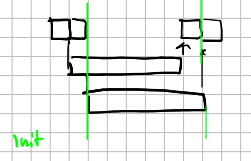
\includegraphics[scale=0.75]{26.png}
\end{center}
Init is the time where every worker has work to do, and finish is the time where the last worker finished working. So the exact formula is
$$T = nw\cdot T_{split} + \frac{m}{nw}\cdot T_{work} + T_{merge}$$
So $\frac{m}{nw}T_{work}$ is the time that needs to happen, found in the sequential computation too, whereas the other two factors are \textbf{overhead}.
$$\hbox{SpeedUp} = \frac{\hbox{Best sequential time}}{\hbox{Parallel time}}$$ but the parallel time depends on the $nw$ so $$\hbox{SpeedUp}(nw) = \frac{\hbox{Best sequential time}}{\hbox{Parallel time}(nw)} \simeq \frac{\not m\cdot \not t_p}{\frac{\not m}{nw}\cdot \not t_p} = nw$$ This not taking into account the overhead. It's a realistic assumption because usually the time splitting the work is very small. But we have to take into account that, in case it's not negligible. $$\hbox{SpeedUp}(nw) = \frac{m\cdot t_p}{\frac{m}{nw}\cdot t_p + \underline{nw\cdot T_{split} + T_{merge}}}$$
%TODO graph sp(nw) over (nw)
\paragraph{Example: Conference Bag} $T_{bag} = t_{bag} + t_{pen} + t_{paper} + t_{proc}$ and with $m$ bags we have $T = m\cdot T_{bag}$\\
We could build a pipeline, a building chain, with 4 people and each person does one task: \begin{list}{}{}
	\item One takes the bag and gives to the next
	\item One puts the pen into the bag and passes it
	\item One puts the paper into the bag and passes it
	\item One puts the proceedings into the bag
\end{list}
So $w_b, w_{pen}, w_{paper}, w_{proc}$ workers. When the first worker has passed the bag, it could begin taking the next bag. Same for the others.
\begin{center}
	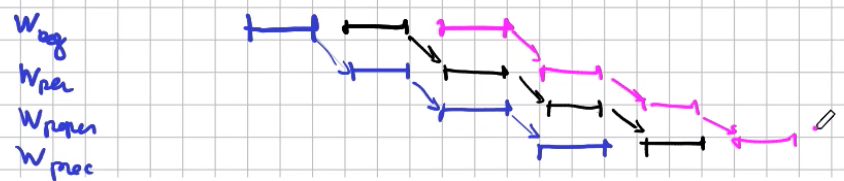
\includegraphics[scale=0.5]{1.png}
\end{center}
So in sequential we have $m\cdot(t_{bag} + t_{pen} + t_{paper} + t_{proc})$, and in parallel per 1 bag we have $t_{bag} + t_{comm} + t_{pen} + t_{comm} + t_{paper} + t_{comm} + t_{proc} + t_{comm}$ with $t_{comm}$ spent passing the bag from one to the other, so total of $m\cdot T_{seq} + m\cdot t_{comm}$. But that's not correct, because we work in parallel: ideally we have a parallelogram of $m\cdot(t_{proc} + t_{comm}$ base, and we require $t_{bag} + t_{pen} + t_{paper} + 3\cdot t_{comm}$ time to get up to speed and "fill the pipeline". But this required time is negligible, and in the end the overall time is given by the base of the parallelogram.
\paragraph{Pipeline} With $m$ tasks and $nw$ stages, with the completion of the stage $i$ required in stage $i+1$. So the output is $f_{nw}(f_{nw-1}(\ldots f_1(x_i)\ldots))$. With $t$ time required for each stage.
\begin{center}
	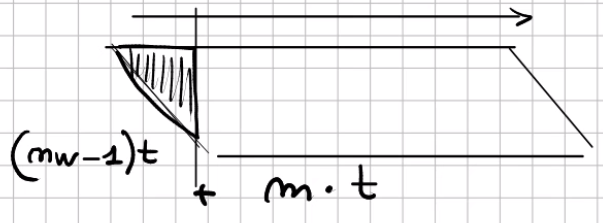
\includegraphics[scale=0.5]{2.png}
\end{center}
We spend $(nw-1)t$ to get the last stage working and $m\cdot t$ time spent by the last stage to complete all the tasks.
$$T_{par}(nw) = (nw-1)\cdot t + m\cdot t$$
$$\hbox{SpeedUp}(nw)=\frac{(nw\cdot t)\cdot m}{(nw-1)\cdot t + m\cdot t}$$
So the higher the $m$ is, the lower is the impact of the time required to get up to speed. So $m >> nw \Rightarrow T_{par}(nw) \simeq m\cdot t$
\paragraph{Throughput} Number of \textbf{tasks completed per unit of time}.
\section{Measures}
On one side we can have \textbf{more speed with more resources} (computing devices).\\
On the other side we can employ \textbf{more complex applications with more resources}. For example more precise computations, so extra resources not for improving the time but to improve the quality of the computations.\\
A recent perspective is to \textbf{aim at computing results with less energy} thanks to parallelism.\\\\
We've seen the SpeedUp($n$) = $\frac{T_{seq}}{T_{par}(n)}$, where the plot has to lie below the bisection of the cartesian graph.
\subsection{Base Measurements}
\paragraph{Latency $L$} Measure of the \textbf{wall-clock time between the start and end of the single task}.
\paragraph{Service Time $T_s$} It's related to the possibility of executing more tasks. It's the measure of the \textbf{time between the delivery of two consecutive results}, for example between $f(x_i)$ and $f(x_{i+1})$\\
Even if $x_i$ and $x_{i+1}$ arrive at the same time, $f$ would still be computing $f(x_i)$ so it'll start computing $f(x_{i+1})$ when it has finished.\\
In a sequential system, $T_s = L$.
\paragraph{Completion Time $T_c$} The latency related to a number of tasks.\\
With a sequential system, we have $T_c = L\cdot m$ for $x_m,\ldots,x_1$ inputs.\\
With a parallel system, we have $T_c\simeq m\cdot T_s$ because we reason at regime.
\paragraph{Example} A 3 stage pipeline, with each node being sequential and with latency $L_i$ for node $i$.\\
At $t_0$ the first stage $N_1$ gets the first tasks and computes it in $L_1$, then $N_2$ computes in $L_2$ and $N_3$ computes in $L_3$ so a total of $t_0 + L_1 + L_2 + L_3$.\\
When the pipeline is filled, $T_s$ is dominated by the longest $L_i$, so $T_s = \max\{L_1, L_2, L_3\}$ and $T_c = \sum L_i + (m-1)T_s$\\
If $m$ is large with respect to $n=$ number of stages, the "base of the parallelogram" would be very long, so $m >> n \Leftrightarrow T_c = m\cdot T_s$
\pagebreak
\subsection{Derived Measurements}
\paragraph{SpeedUp} $$\hbox{SpeedUp}(n) = \frac{T_{seq}}{T_{par}(n)}$$ Could be latencies, service times\ldots depending on what we want to measure the speedup of.
\paragraph{Scalability} $$\hbox{Scalability}(n)=\frac{T_{par}(1)}{T_{par}(n)}$$
\paragraph{Efficiency} $$\hbox{Efficiency}(n) = \frac{\hbox{Ideal parallel time}(n)}{T_{par}(n)} = \frac{\frac{T_{seq}}{n}}{T_{par}(n)} = \frac{T_{seq}}{n\cdot T_{par}(n)} = \frac{\hbox{SpeedUp}(n)}{n}$$
Measures the tradeoff between what you gain with the speedup and the cost of the speedup.
\paragraph{Throughput} $$\hbox{Throughput} = \frac{1}{T_s}$$
\paragraph{Amdahl Law} Taken the total time of a computation, $T_{seq}$, it can be divided into something that can and something that cannot be computed in parallel (for example, dividing the book is a sequential activity). So we can say that\\$T_{seq} =$ serial fraction + parallel fraction and the \textbf{serial fraction cannot be parallelized}. $f\in[0,1]\:|\:f\cdot T_{seq}$ is the serial fraction.
$$T_{seq} = f\cdot T_{seq} + (1-f)\cdot T_{seq}$$
The parallel fraction can be splitted between the workers, but we would have to compute the serial fraction too. By splitting more and more and more, we have that $$\lim_{n\to\infty} T_{par}(n) = f\cdot T_{seq}$$ $$\hbox{SpeedUp}(n) = \frac{T_{seq}}{f\cdot T_{seq}} = \frac{1}{f}$$
So we have a very low upper bound on the achievable speedup. This is referred to as \textbf{strong scaling}: strong meaning using more resources to get the computation faster.
\paragraph{Gustaffson Law} $$\hbox{SpeedUp}(n) = n - S\cdot(n-1)$$ With $S$ being the serial fraction. This comes from the fact that we're considering a different perspective: Gustaffson assumes that the computation increases with the parallelism, something that's called \textbf{weak scaling}: keeping the size of the computation the same for all the concurrent agents that we use. Given $nw$ workers I want $nw\cdot N$ results.

\paragraph{Cores} In modern computers, we have a main memory (slow), a disk (even slower) and the memory is connected to at least 3 levels of cache. At the bottom we have some cores (4, 8\ldots), each one has its own level 1 cache (usually split in data and instruction cache).\\
With an activity with a working set that fills the cache, in case of strong scaling splitting the computation across cores we process less data per core because the size of the problem is the same.\\
With weak scaling, we assume that the data increases so by using more cores we process the same data on all cores but the data grows so we could have extra overhead because of the working set size.\\
We will have patterns of parallel computation that differentiate in how we process the data.
\paragraph{Application as Graphs} The applications can be seen as graphs of sequential nodes with dependencies. The \textbf{work span} model defines two components:
\begin{list}{}{}
	\item Work: the \textbf{amount of time required on a single computing device}, of course respecting the dependencies
	\item Span: the \textbf{length of the longest route} from source to end, in terms of computation time
\end{list}
The maximum speedup is $\frac{\hbox{work}}{\hbox{span}}$, because in every case I need to go from the first to the goal node. I take the longest one because at least the longest path must be computed, and all the rest can be done in parallel and I assume to have enough resources to compute the rest in the time of the span.\\
We \textbf{cannot use this model for reasoning about multiple tasks}, because it does not take into account the parallelism achieved in exploiting different tasks in the same program but \textbf{only takes into account what happens for a single task}. But it can be used, e.g., to reason about a single node of a pipeline.
\section{Patterns}
\textbf{Computations with common and particular shapes and semantics} that can be understood and implemented depending on the situations, not linked to languages and technicalities. Patterns are a useful concepts, allow programmers to reuse experience of other programmers an not reinventing the wheel.\\
Parallel patterns can be of two kinds: \textbf{data parallel}, \textbf{stream parallel}. For each pattern there are more than one name used in literature.
\subsection{Data Parallel Patterns}
\textbf{Parallelism comes from data}: we \textbf{split the data in pieces}, \textbf{compute a set of results} that can be \textbf{combined into a single final result}. The book translation example is a situation where we can apply data parallel patterns. What matters is the latency $L$, we want to be able to provide the result faster once I have the full collection available.\\
The general pattern is:
\begin{list}{}{}
	\item \textbf{Decomposition}
	\item \textbf{Partial results}
	\item \textbf{Recomposition}
\end{list}
Different choices in each phase yield different data patterns.
\begin{multicols}{2}
\subparagraph{Map Pattern} Also called applytoall:\begin{list}{}{}
	\item Decomposition: $\forall$ item of the collection, which is of course the minimum decomposition of a collection
	\item Partial results: $f($item$)$, the result of a function $f$ applied to each item
	\item Recomposition: $\forall$ $f($item$)$, yielding an isomorphic collection to the original one.
\end{list}
\subparagraph{Reduce Pattern} Also called fold:\begin{list}{}{}
	\item Decompose again $\forall$ item of the collection
	\item Partial results: apply a binary function $\oplus(x,y)$ (e.g. the $+$)
	\item Recombination: $\oplus(\oplus(a,b),\oplus(c,d))$
\end{list}
\end{multicols}
\subparagraph{Stencil Pattern} \begin{list}{}{}
	\item Decompose into partially overlapping partitions of the data, e.g. of a matrix or an image
	\item Partial results: the application of a function $f($item$)$
	\item $\forall$ $f($item$)$, again an isomorphic collection
\end{list}
Different kind of problems: overlapping positions will yield the new value, so we have to account for that.
\subparagraph{"Google" mapreduce}
\begin{list}{}{}
	\item Again decompose $\forall$ items
	\item Compute $f($item$) + \oplus($item$_i, $item$_j)$\\
	With $f\mapsto \langle K, V\rangle$ key-value pair and the $\oplus$ function that sums the values of the corresponding keys.
	\item A single item
\end{list}
What I apply to each item is an $f$ that maps to $\langle$key, value$\rangle$ and $\oplus$ applies the sum to each value.\\
For example in a document, $f($word$)=\langle w,1\rangle$ and $\oplus(\langle w_k,v_1\rangle,\langle w_k,v_2\rangle) = \langle w_k, \oplus(v_1,v_2)\rangle$\\
"The lesson given by the professor", $f$ will output $\langle$the, 1$\rangle,\langle$lesson, 1$\rangle$\ldots and $\oplus$ will for example output $\langle$the, 2$\rangle$.\\
We can apply the map function over all the data distributed in various databases, for example.\\
This is \texttt{map(f)} and \texttt{reduce($\oplus$)}, but we want something like \texttt{map(reduce($\oplus$))}. Combining elementary patterns to achieve more complex results. Like two nested \texttt{for}s.\\
So I want building blocks, something that guarantees correctness of implementation that can be used to build upon. For example \texttt{map(function<A(B)>, collection<B>)}\\
So build a bag of tools that we can combine to undertake common situations with good efficiency, speedup, scalability\ldots
\subsection{Stream Parallel Patterns}
Stream of data, flowing in time. In data parallel we process a data collection, while in stream parallel \textbf{we don't have data appearing all at the same time}. So \textbf{stream as a collection with items appearing at different times}. We want to take the single items and try to process in parallel, parallel execution of $f$ over different items of the stream.\\
What matters is the service time $T_S$, to be able to sustain the flow of data and process the next available item as soon as it arrives.
\paragraph{Pipeline}
\begin{center}
	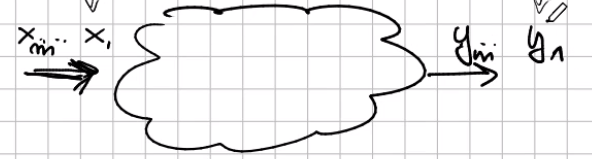
\includegraphics[scale=0.5]{3.png}
\end{center}
Inside the pipeline we have $f_1\rightarrow f_2\rightarrow\ldots\rightarrow f_k$ with each $f_i$ corresponding to a phase, with $f_i$ taking input from $f_{i-1}$.\\
So $x_i\mapsto f_1(x_i)\mapsto f_2(f_1(x_i))\mapsto \ldots$, and the parallelism is in the computation of different phases of different items (much like what we've seen with the CPU fetch-decode-execute pipeline).
\begin{center}
	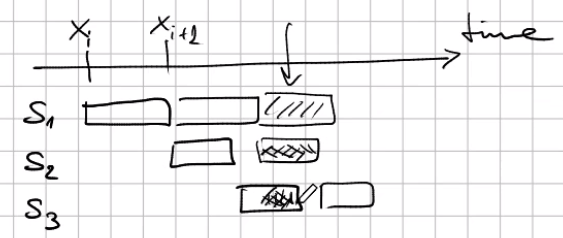
\includegraphics[scale=0.5]{4.png}
\end{center}
\paragraph{Farm}
We have a number $nw$ of instances of the same function $f$ each processing one single item.
\begin{center}
	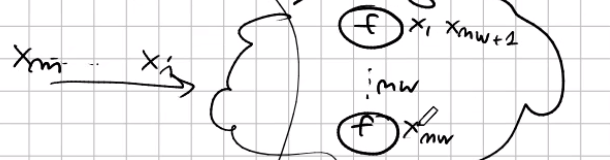
\includegraphics[scale=0.5]{5.png}
\end{center}
We have no interference between computations of $x_i,x_j$ with $i\neq j$, no need for synchronization.\\\\
The completion time $T_C$ is $\simeq m\cdot T_S$ (number of tasks times service time). In the sequential stages, $T_S = L$. This means that given a stream of item to be computed in a parallel fashion, and I want to increase $T_C$ or $T_S$, the I would need to decrease the latency of the stages in my pipeline or the workers in my farm.\\
If we have pipe(seq($f$), seq($g$)) then by decreasing the latency of $f$ we will already improve the performances of the overall computation. Keep in mind that \textbf{not every kind of computation can be parallelized}.
\paragraph{Two Tier Model} Let's assume a grammar of patterns.\begin{list}{}{}
	\item Pat = Seq(f) $|$ DPP $|$ SPP
	\item DPP = Map(Pat) $|$ Reduce(Pat)
	\item SPP = Farm(Pat) $|$ Pipe(Pat, Pat)
\end{list}
This defines parallel computations and we aim at assuring that this can be done, a way of implementing this. So\begin{list}{}{}
	\item Map(Pipe(Seq(f), Seq(g)))
\end{list}
can be a data parallel computation where on the single item we compute a 2-stages pipeline of $f$ and $g$. But each element of the map is given to a single pipeline, or each pipeline receives a single item, so the stream parallelism is useless.
\begin{list}{}{}
	\item Farm(Map(Seq(f)))
\end{list}
Here we have a stream of items that will be processed by a Farm, each item splitted by Map and processed. This can deliver the result faster and access the next item.\\
So Data parallel with Stream parallel is not very good, Stream parallel with Data parallel is better: \textbf{two tier model}.\\
So we have an initial part of the pattern which is Stream Parallel, the second part is Data Parallel and eventually the last stages (the leafs of the tree) which are sequential.
\paragraph{Parallel Design Patterns}
Also called \textbf{algorithm skeletons}: programming abstraction that model some pattern. The programmer has a framework, libraries, languages and that includes algorithm abstractions.
\subsection{Composing}
These are building blocks, so we can \textbf{compose} them. Let's see how that works and what are the expected performances.
\subsubsection{Pipeline}
We have a number $k$ of stages for $m$ tasks: Pipeline$(s_1,\ldots,s_k)$ meaning that this is a composition yielding $s_k(\ldots s_1(\:)\ldots)$
$$\hbox{Input stream}\longrightarrow s_1\rightarrow\ldots\rightarrow s_k\longrightarrow\hbox{Output stream}$$
With each $\rightarrow$ being a stream $s_i\rightarrow s_{i+1}$ and each $s_i$ taking input from $s_{i-1}$.\\
The latency of the pipeline is the sum of the latencies of the stages $$L(\hbox{Pipeline}(s_1,\ldots,s_k)) = \sum_{i=1}^k L(s_i)$$
We do not consider the time required to pass input to the next stage, $t_{comm}$, which would be based on size, nature of the computation\ldots\\
The steady state is when all the stage are "filled": the longest of the stages will dominate the service time $T_S$
$$T_S(\hbox{Pipeline}(s_1,\ldots,s_k)) = \max_{i=1}^k\{T_S(s_i)\} = \max_{i=1}^k\{L(s_i)\}$$
The completion time is $T_C$
$$T_C(\hbox{Pipeline}(s_1,\ldots,s_k)) = \left(\sum_{i=1}^k L(s_i)\right) + (m-1)\max_{i=1}^k\{L_i\}$$
and when $m >> k$ we can approximate it with
$$T_C = mT_S$$
because the number of tasks required, the "base of the parallelogram", will dominate the number of workers, the "height of the parallelogram".\\
What if I want to achieve a given performance? For example, given a Pipeline($S_1, S_2, S_3$) where $S_1$ and $S_3$ both take 1s and $S_2$ takes 2s, and we want a $T_A=T_S=$ 1s. We can't do much, by necessity $T_S=\max\{$1s, 5s, 2s$\}=$ 5s, and in general I don't know what's inside each stage of the pipeline so I can't perform optimization inside those. In this case, we can take the \textbf{bottleneck}, the slowest stage ($S_2$), and shorten the $T_S$ by adding a farm in its place: Pipeline($S_1$, Farm($S_2,\:$), $S_3$). This computes the very same result:
\begin{list}{}{}
	\item With the first form, Pipeline($S_1, S_2, S_3$), we compute $S_3(S_2(S_1(x_i)))$
	\item With the second form, Pipeline($S_1$, Farm($S_2,\:$), $S_3$), we compute $S_1(x_i)$ which delivers the result to the scheduler of Farm($S_2,\:$), where each worker computes $S_2$ and the scheduler selects which worker will compute it yielding $S_2(S_1(x_i))$. The farm then delivers the result to $S_3$, which will output the final result $S_3(S_2(S_1(x_i)))$
\end{list}
This works well if every timing remains the same. But if a worker in the $S_2$'s farm takes longer we may encounter a situation where $S_3$ receives a $x_{i+1}$ before receiving $x_i$. This may be irrelevant or be unacceptable depending on the kind of application. With 5 workers in the farm, we end up with $T_S=$ 1s.\\
Another approach would be to consider the original pipeline as a single task computing $P(x) = S_3(S_2(S_1(x)))$ and building a farm with workers that each compute $P$. $P(x)$ has a latency $L = 1+5+1 =$ 7s, so with a farm composed by 7 $P$ we have a $T_S =$ 1s.\\
Which is better depends:
\begin{list}{}{}
	\item Pipeline($S_1, S_2, S_3$) has $T_S=5$s and $nw=3$
	\item Pipeline($S_1$, Farm($S_2,5$), $S_3$) has $T_S=1$s and $nw=7$ ($+2$ for $E$ and $C$)
	\item Farm($P, 7$) has $T_S=1$s and $nw=7$ ($+2$ for $E$ and $C$)
\end{list}
Noting that each farm adds $2$ workers. So by refactoring with the farm we need more workers, which can be a decision point in implementing this kind of refactoring.
\paragraph{Boundary Conditions} We have to take into account the \textbf{interarrival time} $T_A$, time spent to get another item from the input stream, and the \textbf{interdeparture time} $T_D$, the time spent to get another item into the output stream.\\
Let's suppose that $L(s_i) = i$ seconds, so ideally $T_S = k$ seconds: we process 1 item each $k$ seconds. If $T_A > L(s_i)$ we have to wait the second item when I finish processing the first, same thing for the next after the second: the interrarival time looks like an interstage between $s_{i-1}$ and $s_i$.\\
$T_D$ behaves at the same way: we have to wait that $T_D$ finishes before giving it out output, behaving like an interstage.\\
So the previous behavior, analyzed before, happens $\Leftrightarrow T_A<T_S$ and $T_D<T_S$ \textbf{something that we have always to take into account}.
\subsubsection{Farm}
Sometimes we denote as Farm$(s, nw)$, otherwise we omit the number of workers and simply write Farm$(s)$.\\
We assume to know $L_w$ and $T_w$ of the workers. We have some scheduler (\textbf{emitter} $E$) that distributes the items from the input stream to the workers, and a gatherer (\textbf{collector} $C$) that gets the results from the workers and delivers them to the output stream. Those can simply be data structures: queues, for example.
$$L(\hbox{Farm}(s,nw)) = t_E + L_w + t_C$$
This can appear as a pipeline of three stages, where the Emitter produces to the second stage (the workers) which produce to the third stage (the Collector)
$$T_S(\hbox{Farm}(s,nw)) = \max\left\{t_E, \frac{T_w}{nw}, t_C\right\}$$
We assume to have $m$ tasks
$$T_C(\hbox{Farm}(s,nw)) = m\cdot T_S(\hbox{Farm}(s,nw))$$
If we take into account the boundary conditions
$$T_S=\max\{T_s(\hbox{Farm}()),T_A,T_D\}$$
What if we want to achieve a given performance? Compute a $nw$ suitable to achieve a wanted performance by inverting the very same formulas.\\
With a target $T_S = T_A = 1$s
$$T_S = 1\hbox{s} = \max\left\{t_E, t_C, \frac{10\hbox{s}}{nw}\right\}$$
But $t_E,t_C$ are negligible so $$\frac{10\hbox{s}}{nw} = 1\hbox{s} \Rightarrow nw = 10$$
\subsubsection{Map} The map data parallel pattern is composed by three main phases:
\begin{list}{}{}
	\item Split: divide the collection into sub collections, a \textbf{set of subcollections}
	\item Map: compute the \textbf{set of subresults}
	\item Merge: produce the final \textbf{collection results} (usually in the same shape as the input collection)
\end{list}
With $m$ dimension of the collection and $t_f$ to compute the function of the map $$L(\hbox{Map}) = \frac{m\cdot t_f}{nw} + t_{split} + t_{merge}$$
$t_{split}$ and $t_{merge}$ are non-negligible in distributed architectures, but are negligible in shared-memory architecture.
$$T_S(\hbox{Map}) = L(\hbox{Map})$$
No concept of $T_C$ because the map is applied to a single collection.\\
If I have multiple collections we can consider a 3-stage pipeline composed by a splitter node as $s_1$, the map as $s_2$ and merger node as $s_3$, giving
$$T_S=\max\{t_{split}, t_{map}, t_{merge}\}$$
$$t_{map} = \frac{m}{nw}t_f$$
The structure of a map resembles that of a farm, thus to increment the performances we can increment the number of the workers that implement split/merge operations. This requires synchronization between the workers of the split/merge operations in order to avoid the repetition of elements.
\subsubsection{Reduce}
From a vector we want to output the sum: a scalar from a collection. We split in $t_{split}$, then each of the $nw$ workers applies the function $\oplus$ to its subcollection in $\frac{m}{nw}t_\oplus$ and finally we merge in $nw\cdot t_\oplus$ because we have to compute $\oplus$ over all the $nw$ subresults.
$$L=t_{split} + \left(\frac{m}{nw}-1\right)t_\oplus+(nw-1)t_\oplus$$
$$T_S = L$$
With multiple collections, same argument as before
$$T_S = \max\{\ldots\}$$
But the computation can be organized in a logarithmic tree, too. We would have $\log_2(m)$ phases each with half the activities of the previous phase.\begin{center}
	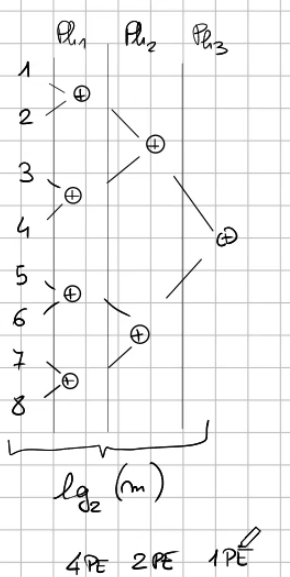
\includegraphics[scale=0.5]{6.png}
\end{center}
But we have efficiency 1 only in the first phase, then half, then one fourth\ldots
$$L=t_{split}+\lceil\log_2 m\rceil t_\oplus$$
provided that $nw \geq \frac{m}{2}$. If we use threads, the split phase is just telling the threads what they have to do, then we merge with a simple loop.
\subsubsection{Stencil}
For example computing the average of three neighbor items in a vector, with \textbf{necessary boundary conditions}.\\
Split phase that produces for example two halves of the vector: when computing the right extreme of the first half, I need to add the first item of the second vector, same with the left extreme of the second half: we have some shared positions. No problem when reading, the \textbf{problem arises when we write the shared position}.
\begin{list}{}{}
	\item A first solution would be to \textbf{use 2 buffers}: we read from a buffer and write to another buffer, and we swap the buffer before restarting such that we use the new values to read and the old values to write.
	\item Another solution is to \textbf{use a small buffer to host modified values in the neighborhood}. The result is kept in a buffer before being written to the array. The buffers are written when we move to such a position that the edited previous position are no longer read: the buffer would need to contain at most half the radius of the stencil operation.
\end{list}
$$L(\hbox{Stencil}) = t_{split} + \frac{m}{nw}t_{stencil} +t_{merge}$$
Where $t_{stencil}$ includes buffer management with the second solution and $t_{merge}$ includes swapping the buffers in the first solution.
\paragraph{Composition} Given a Pipeline($s_1,s_2,s_3$) with $s_i$ sequential, $s_2$ may be data parallel (map), $m$ stream items and each being a vector of $k$ items.
$$L = L_1+L_2+L_3$$
$$T_S=\max\{L_1,L_2,L_3\}$$
$$T_C\simeq m\cdot T_S$$
$s_2$ is sequential but can be turned into a map, takes $L_2$ so I can imagine $t_f \simeq \frac{L_2}{k}$
$$T_S(\hbox{Pipeline}) = \max\left\{L_1,L_3,\frac{L_2}{nw_{\hbox{map}}}\right\}$$
Note how the latency decreases. This of course \textit{if} $s_2$ can be turned into a map: I \textbf{need to be able to check the code}.\\
Another approach, as we saw before, is this: given that $s_2$ is the slowest stage, we can use a Farm$(s_2, nw_{\hbox{farm}})$. However in this case latency stays the same.
\paragraph{Single Owner Computes rule} Is a more general pattern: each part of the data structure has a \textbf{single owner} who is \textbf{in charge of performing the computing} of the new values in that particular part.
\section{Technicalities}
\subsection{Threads}
To create a thread using the \texttt{std::thread} library we use \texttt{auto tid = new std::thread(function, ...);} which starts a new flow control that runs the passed function. We are used to writing instructions sequentially, now we \texttt{fork} another flow of computation: we get two flows that are executed together \textbf{in the same address space}, so \textbf{the new thread inherits all the memory of the original thread}.\\
Correctly handling the threads is fundamental, e.g. by \texttt{join}ing them at the end of a computation or \texttt{detach}ing them if needed: \textbf{detach separates the thread from the process} allowing the \textbf{execution to continue independently} (\texttt{detach}ed threads cannot be \texttt{join}ed).\\
Another useful method is \texttt{yield()}, which signals to the scheduler that this thread can release the processor and be rescheduled later. This is useful in non-timesharing contexts or when a thread describes a very long computation.
\subsection{Synchronization}
Two fundamental approached: \textbf{controlling data sharing} (\texttt{mutex}es) and \textbf{waiting on events} (condition variables).
\paragraph{Mutexes} \texttt{std::mutex} objects are used to implement \textbf{mutual exclusion} with \texttt{lock} before and \texttt{unlock} after a certain block of code that needs to be executed by just one thread at a time. Thus \texttt{mutex} objects need to be shared.\\
Often the critical section that needs to be protected is very small and lasts for a small block of data. \texttt{std::lock\_guard} mechanism can be declared having a \texttt{std::mutex} as parameter. It tries to acquire the mutex's lock when declared and will automatically release it when its scope ends (by its object destroyer).\\
Last mechanism is the \texttt{std::try\_lock} function: it returns immediately with \texttt{true} if the lock has been acquired, \texttt{false} otherwise.
\paragraph{Condition variables} \texttt{std::condition\_variable} objects provide the method \texttt{wait} that takes a \texttt{mutex} and optionally a predicate as parameters, and the methods \texttt{notify\_one()} and \texttt{notify\_all()}.\\
We call the \texttt{wait} on some shared data, waiting for some kind of event. Once we call the \texttt{wait}, the thread is asleep and releases the lock on the mutex until some other thread calls one of the \texttt{notify} methods (and the relative \texttt{unlock}!).\\
With \texttt{notify\_one} only one of the waiting threads is put in the ready list, whereas with \texttt{notify\_all} every waiting thread will be put in the ready list. When a thread is awaken by a notify method, it will try to reacquire the lock. Once a thread is awake and has reacquired the lock, \textbf{it needs to re-check the condition it was waiting} because there's no guarantee that, due to scheduling, the condition has not been invalidate between the \texttt{notify} event and the thread actually being put into execution. So usually the \texttt{wait} are put inside a \texttt{while(condition)} loop.
\subsection{Async}
\texttt{std::async} are a bit different. When instantiating an \texttt{std::thread} it starts and forks the execution of the program. For \texttt{std::async} we simply tell the system that it \textit{can} execute that portion concurrently, and it will be executed in a thread if and only if a thread is available. An async returns a \texttt{future} that can be used to know the status and return value of the computation.
\subsection{Packaged Tasks}
\texttt{std::packaged\_task} decouples the moments of having a function to call from the moment of calling that function. With \texttt{get\_future} we can get the future relative to the packaged task and use it. To compute the packaged task we call it passing the arguments, e.g. the packaged task of the function \texttt{t1 func(t2);} is \texttt{auto pt = new packaged\_task(func);} has future \texttt{auto future<t1> ft = pt.get\_future();} and can be called with \texttt{pt(arg);} with \texttt{arg} of type \texttt{t2}. The result can be obtained with \texttt{t1 res = ft.get();}.
\subsection{Promises}
\texttt{std::promise} can be used in two ways: using its future like before or call \texttt{set\_value} on it. They can be viewed as \textbf{placeholders}.
\subsection{Overhead}
Standard computer of course have a processor and a memory, connected by some kind of bus. This bus represents a bottleneck (the \textbf{Von Neumann Bottleneck}). We can improve by having two memories: an instruction memory and a data memory.\\\\
By exploding the Von Neumann model a bit, we have a \textbf{main memory}, a number of \textbf{cache} levels faster and smaller going from the main memory to the processor, and the \textbf{processor}. Usually the last level of cache, closest to the processor, takes 1 or 2 $\tau$ (clock cycles) to perform the operations, while the main memory takes around 80 to 100 $\tau$. This follows the \textbf{locality principle} which is divided into \textbf{spatial locality} (if a given address $i$ is accessed, then it's likely that addresses $i+1$ and so on will be accessed soon)  and \textbf{temporal locality} (an accessed address is likely to be accessed again soon), enabling the concept of \textbf{working set} (the set of addresses that are likely of being accessed in a small amount of time).\\\\
In a multi-processor system, e.g. an 8-core processor, we have some levels of cache that are shared between cores (ideally the higher levels, closer to the main memory) and some that are independent per-core. In this case, \textbf{a shared variable should keep the same value even when we have independent caches}. This is achieved by an hardware component that implements the \textbf{cache coherence protocol}. This requires some time, of course. This is achieved by a bus (\textbf{snoopy bus}) that is placed between the last level of shared cache and the first level of independent caches. This bus detects operations on independent caches and propagates accesses to shared variables. Other systems implement a \textbf{directory of shared data} and polls it whenever shared data is accessed. The key takeaway here is that \textbf{there is something that we need to do to keep the copies consistent}.\\
This \textbf{cache coherency protocol} is applied to cache lines, which are the minimal units of operations on caches. So whenever the line containing the shared variable is changed, all the line is moved in all the other places. So it at least has to access the first shared level of cache, if not going up until the main memory. This has to be made for the whole working set of the thread.
\paragraph{Example} If we use the stencil pattern to implement matrix multiplication, we may have a \textbf{cache line that is "split" between} two portions of the data, thus \textbf{two threads}. Each time a value is written inside that line, the cache coherence protocol runs. In a stencil computation this makes sense.\\
In, e.g., a map operation we may have a vector where $x_i^t = f(x_i^{t-1})$ performed for several $t$s. If this cache line is shared with another core, this may trigger the cache coherence protocol for all the other items that may be never used, resulting in the \textbf{false sharing problem}. We must try to avoid as much as possible this situation, because \textbf{this adds significant overhead} to the computation.\\
We use \textbf{padding techniques} that adds pad values to the original vector such that the culprit cache line is filled with dummy values to avoid sharing it with other cores.\\\\
Another overhead problem occur when \textbf{a thread is moved from a processor to another}. The receiving processor in general does not possess any element of the incoming thread working set in its cache levels.\\
This switch is decided and performed by the operating system, but this decision may not be optimal for some programs, especially if we want to harness the full potential of all the cores on a machine. We can \textbf{force it to not perform this operation by pinning the threads} to some particular core, by specifying its identifying number.\\\\
Another source of overhead is \textbf{communication}, e.g. between stages in a pipeline: each stage spends some time to receive and some time to send, other than the time spent computing. With threads this may be ignored, because those read and write in shared memory, but this may not be negligible in distributed systems across a network. Even on fast networks with $1\mu s$ latency, this would still be 3 orders of magnitude greater than the clock cycle time. This could result in receive and send times greater than the computation time. Sending data in the end is simply tell the network adapter the address of the data and the order. At this point, instead of waiting, the node could simply begin performing the next computation and be interrupted when the data transfer is completed (and handle errors if there are). Another solution is to have three threads and implement a kind of pipeline where the first thread receives into a buffer, the second thread computes in another buffer and the third thread sends from another other buffer. At the next stage, the first thread computes from its buffer, the second sends its result and the third receives inside its buffer. At regime, we spend $\max\{t_{rec}, t_{comp}, t_{send}\}\cdot n$ time. This allows to hide communication times if and only if $t_{comp}$ is larger than the other two times (receive and send).\\\\
We mention this technique to be useful in clusters of network-connected workstations, but a similar situation may be present in CPU-GPU communication. GPUs are accelerators, thus are connected to the processor by some kind of bus (the PCIe bus), and have their own memory. Let's say we have a map($f$) with a time-consuming $f$, on a huge $v$. We can \textbf{move $v$ to the GPU's memory}, the \textbf{GPU kernel computes} map($f$) over $v$ and the result $v'$ is then brought back to the CPU memory. The key point here is that we have to \textbf{move data to and from the GPU memory}. GPUs provide 1 or 2 \textbf{DMA Engines} that are in charge of this GPU-CPU data transfer. This DMA engines work like the NIC mentioned before: and address is written on the bus and it will handle read/write operations without impacting performances.\\
Given a vector $v$ and a map to be computed, we can consider chunks of the vector such that the computation time over the chunks is $t_f\simeq t_{comm}$ the communication time. This technique is very common and can be achieved in two ways: moving data from CPU to GPU explicitly or use \textbf{streams} which are abstractions, streams of operations. Streams can be of three types: move CPU$\rightarrow$GPU, move GPU$\rightarrow$CPU or compute. We setup three streams.
\paragraph{Overhead related to memory allocations} New objects are created when instantiating inputs and results, for example. This requires allocating memory in the heap, with corresponding \texttt{malloc}s and \texttt{free}s. So we may need to be smarter, with solutions that work on thread-level memories, small heaps where to allocate objects and releasing when no more needed.\\
As for threads, the operation \texttt{new} which creates a new thread, and \texttt{join} which waits for the completion of a thread, of course both take some time. There is a \textbf{tradeoff} between the time spent to setup the parallel activity and the time earned from it. If the time spent computing by a thread is smaller than the time required by creating and joining it then it is pointless to perform that computation in another thread.
\subparagraph{\texttt{jmalloc} library} Used in BSD systems, FireFox and Facebook among others.\\
It manages \textbf{chunks of memory} called \textbf{arenas}, distributed in a round robin way per thread with each thread using one arena. A metaarena is used a common place.\\
Arenas A1, A2,\ldots, Ak are assigned in round robin to th1, th2\ldots. When some data comes from an arena, and we free that data we free the original arena not the local one. \texttt{jmalloc} has its own API, but other than that it uses the classical API: \texttt{malloc} and \texttt{free}, same as stdlib.\\
Taking a normal program \texttt{a.out}, with \texttt{./a.out p1 \ldots pk} we will go with \texttt{malloc} and \texttt{free} of the stdlib. If we prefix with \texttt{LD\_PRELOAD=libjmalloc.so ./a.out p1 \ldots pk} then \texttt{malloc} and \texttt{free} will be loaded from the \texttt{jmalloc} library.
\subsection{Implementation of Patterns}
We spoke about stream (pipeline, farm) and data (map, reduce, stencil) parallel patterns. Let's discuss some general techniques to implement them. The basic structure of a pipeline is: an inputstream, outputstream and a number of stages implementing functions $f_i$. So the parameters are $\{f_i, is, os\}$ , and our tools are threads/asyncs etc. from C++.\\
There are two main approaches to the implementation: \textbf{template based} implementation and \textbf{macro data flow} implementation (MDF).
\paragraph{Template Based} We assume that for each pattern (pipelines, farms, maps, stencil\ldots) we have a template, which is composed by three parts:
\begin{list}{}{}
	\item a \textbf{target architecture}, e.g.: shared-memory multi-core, cluster/network of workstations, cloud\ldots
	\item \textbf{concurrent activity graph}, a graph representing concurrent activities with their communication channels
	\item \textbf{performance modeling}
\end{list}
\textbf{An example is a template of a pipeline} in a shared-memory multi-core environment: template(pipeline, SMmulticore). We have two choices:
\begin{list}{}{}
	\item Take a number of \textbf{concurrent threads} linked by communication channels like queues. Given $m$ stages, we have $m-1$ queues and the performance model is speedup$(m)\simeq m$ when each stage has circa the same $t_S$.
	
	\item Use a \textbf{queue} to pile up tasks which are $\langle f, x_i\rangle$ pairs: $f$ represents the function that needs to be computed on $x_i$. We have a number of threads, each takes a task from the queue, computes $f(x_i)$ and puts into the queue $\langle g, f(x_i)\rangle$ with $g$ representing the next stage of the pipeline that needs to be computed.\\
	There are two main issues: the queue represents a bottleneck and we need to handle the ordering of the tasks, but both can be tackled in various ways. For example, splitting the queue in a set of queues or adding the information $i$ to the pair put in the queue to handle the ordering.\\
	Performances of this model are very different: we don't have the limitation of having all tasks with same $t_S$. Provided to have a sufficient $t_A$ (interarrival time) and given $nw$ \textbf{workers}, not stages, we have speedup($nw) \simeq nw$. With $nw$ being the number of threads used, the workers, we have $nw+2$ stages (the input and output stages count!)
\end{list}
We can consider another alternative
\begin{list}{}{}
	\item Take a number of parallel activities, with a round-robin schedule delivering data and with a sorter gathering and sorting the results. The scheduler tags each task with the appropriate number, so that the sorter can correctly sort the results.\\
	We have $nw$ concurrent activities, and thus $nw$ queues plus the queue of the sorter. With a small enough interarrival time $t_A$, we can achieve a speedup($nw$) = $nw$
\end{list}
So on the same architecture we can implement a pipeline in at least three different ways. What if we change architecture, e.g. from SMmulticore to COW (cluster of workstation)? A COW is a cluster of multicores, basically, so we can use any template seen before. Each workstation is a stage and the communication channels are something like TCP/IP sockets, achieving once again a speedup circa the number of stages.\\
Another template is to have each workstation provide a number of workers, with a scheduler queue and a sorter queue as output like the last template seen earlier. These workstation work in a pipeline, with input/output communication channels, and each implementing an array of worker threads.
\begin{center}
	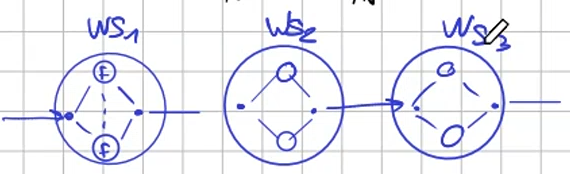
\includegraphics[scale=0.5]{27.png}
\end{center}
In this example, $t_S\simeq\frac{\max\{t_1,t_2,t_3\}}{nw}$ and the main source of overhead is in the scheduling/gathering part in each of the workstations. But each workstation orders the results that will be generally ignored, what's important is to maintain the arrival order in the final output. So we can take away the sort at the end of each workstation, ending up with something like $t_1\simeq t_2 = t_{\hbox{scheduling}} + \frac{t_f}{nw}$ and $t_3 = t_{\hbox{scheduling}} + \frac{t_f}{nw} + t_{\hbox{sorting}}$, but given that $t_S=\max\{t_1, t_2, t_3\}$ we still have overhead. We can decouple the sorting stage outside the last workstation and add a sorting stage, with the only task of sorting what it gets.\\\\
The key idea is that \textbf{template based implementation provide a kind of library} with a number of items made of $\langle$pattern, graph, hardware, performance model$\rangle$ from which we can select the best template suited for our specific situation.
\paragraph{Macro Data Flow} With \textbf{data flow} we denote models where the \textbf{order of the computations are dictated by the flow of data} rather than the program counter.\\
We are used to flows where the order of the instructions is dictated by the program counter. In data flow, we execute instructions in the order dictated by how data flows, meaning that operations are executed only when the required data is available. An example: if we want to compute $(a+b)\cdot(c-d)$ with \textbf{imperative style} programming the evaluation would go something like: \begin{lstlisting}[style=myC]
temp1 = a+b;
temp2 = c-d;
res = temp1*temp2;
\end{lstlisting}
With the program counter pointing to \texttt{1} at $t_1$, to \texttt{2} at $t_2$ and so on. With \textbf{data flow} we have a radically different approach we have a tree of operations:
\begin{center}
	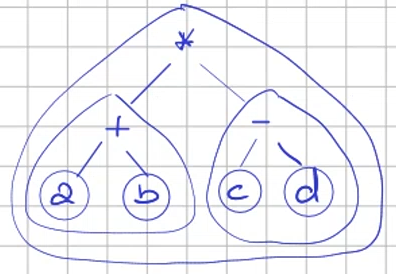
\includegraphics[scale=0.5]{28.png}
\end{center}
To compute $*$ I need the $+$ and $-$ trees, and each tree requires computing some other values\ldots In a sense, the syntax dictates the order of operations. So we interpret this as having, for each operation, a node specifying the function, input arcs and output arcs. E.g. $\langle+, a, b, out\rangle$
\begin{center}
	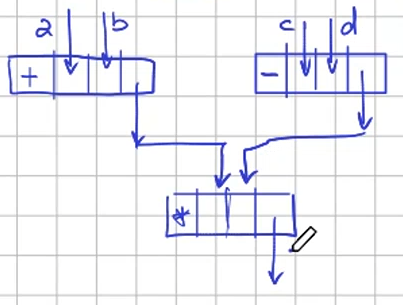
\includegraphics[scale=0.5]{29.png}
\end{center}
Each arc possess a token that signals its availability. If we start with $a$ and $c$ available, neither $+$ nor $-$ instructions are executed. Once $b$ is available, the $+$ action becomes \textbf{fireable}. The macro data flow graph \textbf{gathers all fireable operations and executes them}. The \textbf{execution empties the input tokens of an action and fills its output token}(s), thus becoming a non-fireable action. Given a set of fireable actions, we can \textbf{execute those in every order we want}.\\
In \textbf{\textit{Macro} Data Flow}, instead of considering action nodes composed by input tokens, output tokens and simple functions, we instead consider the possibility of having entire portions of code, methods, as the computable part of the node. Given a program, which uses some patterns e.g. pipe(seq, farm(seq), seq), its pattern tree is compile into a \textbf{MDF graph}. We have a \textbf{graph repository} and a \textbf{pool of executors}. Any time I have some input data, I \textbf{create a copy of the MDF graph and place it in the repository with the instantiated input tokens}. Each executor performs a loop where they get the fireable instruction, computes the action and delivers the output tokens where they need to go.
\begin{center}
	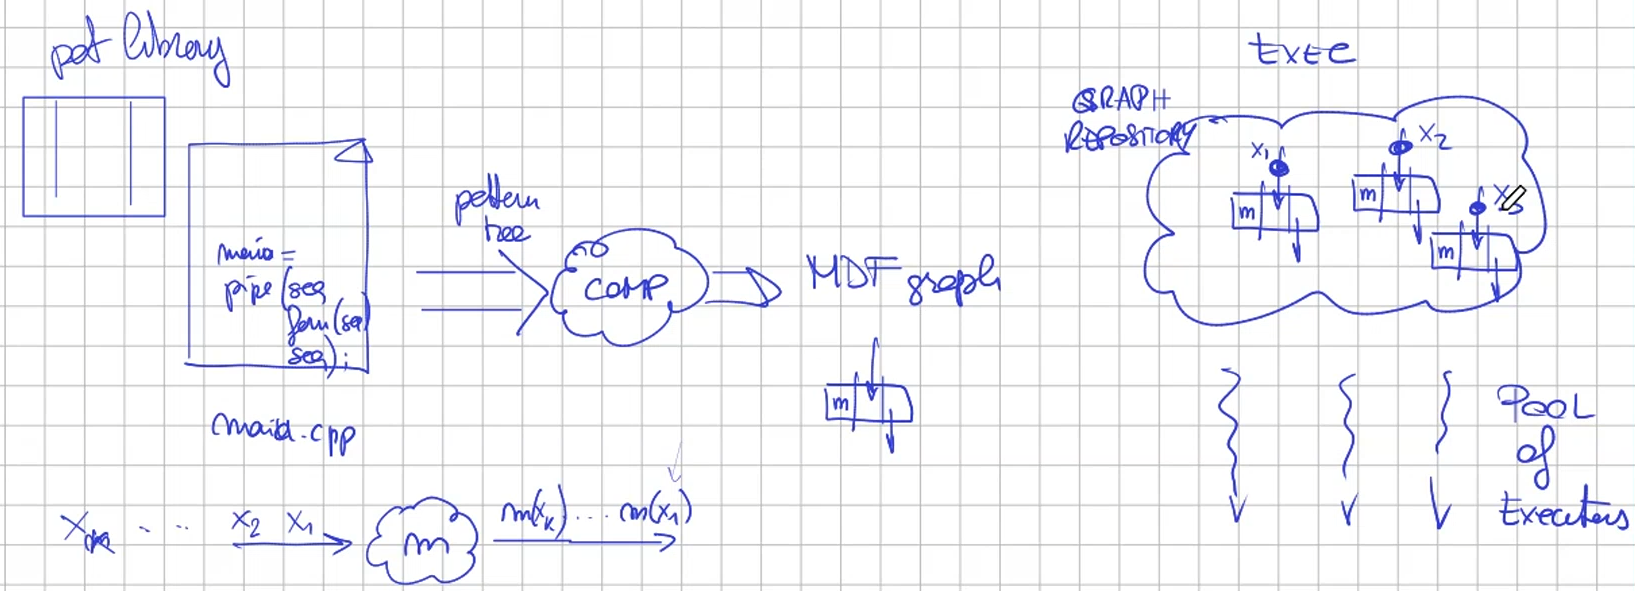
\includegraphics[scale=0.4]{30.png}
\end{center}
The key is the compilation of the parallel patterns.
\begin{center}
	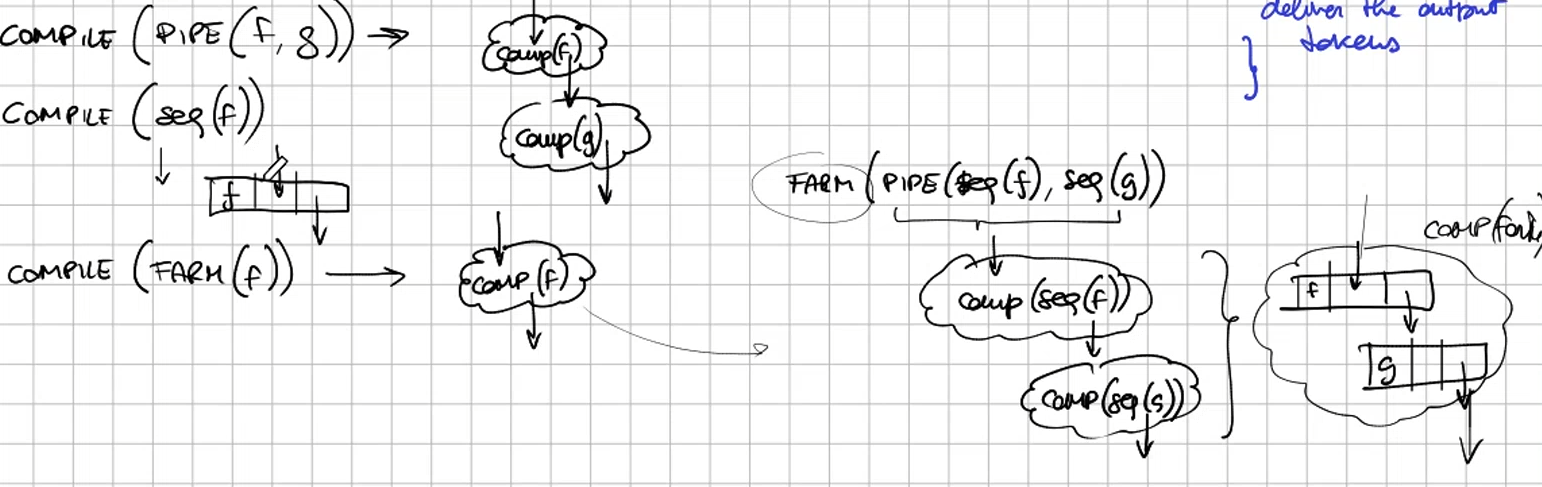
\includegraphics[scale=0.4]{31.png}\\
	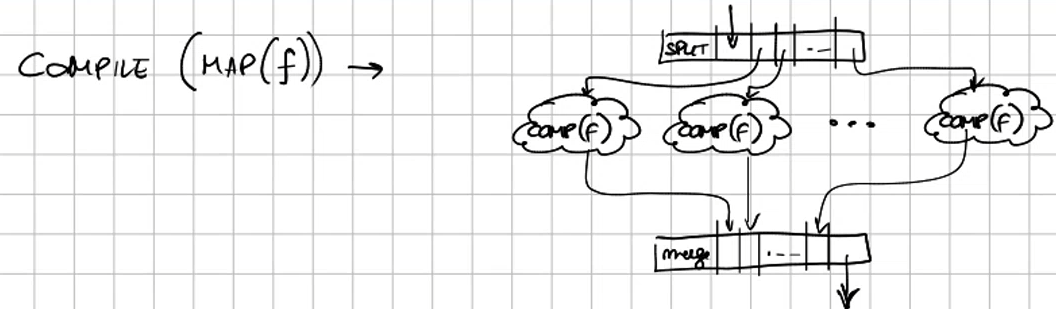
\includegraphics[scale=0.5]{32.png}\\
	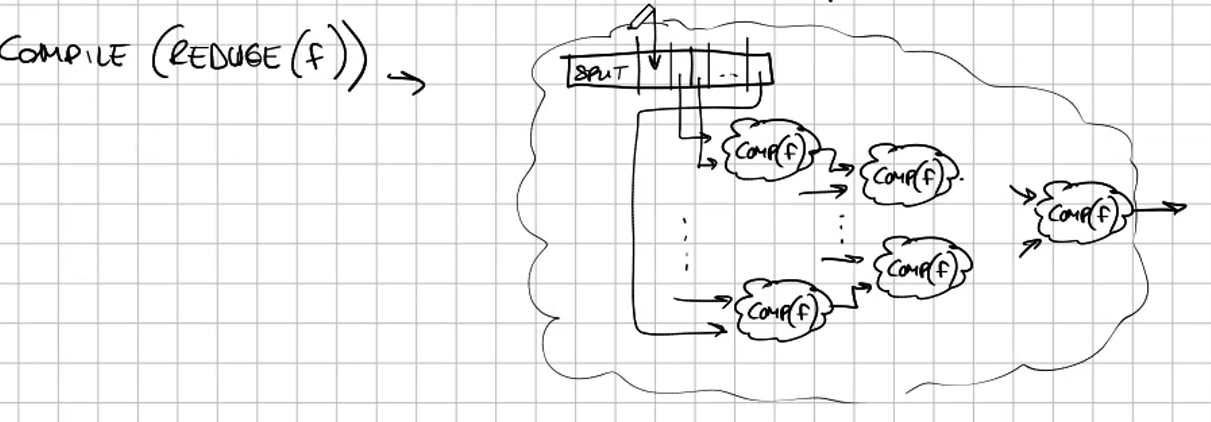
\includegraphics[scale=0.5]{33.png}
\end{center}
MDF can issue some problems. First, the concurrency over the repository of course.\\
Another problem is the result tokens delivery: each graph can need input tokens coming from different computations, and such we need to handle it.\\
Another thing is maintaining the list of fireable instructions. For efficiency reasons, we maintain a \textbf{counter} inside the node (along with the function, the input tokens and the output destinations). This counter tells how many input tokens are needed to compute the function, and each time a token becomes available the counter is decreased by 1. When the counter is 0, then the instruction is fireable so the last thread who delivers the final input token is in charge of putting the receiving node in the fireable list.\\
Another is the out stream must be efficiently maintained, possibly reordering the results when needed.\\
Finally, we need to take into account some kind of graph ID to distinguish of course the various copies of the same graph.\\
So a node would in the end by composed by:
\begin{list}{}{}
	\item \textbf{Graph ID}, identifying the copy of the graph
	\item \textbf{Instruction ID}
	\item The \textbf{function} to be computed 
	\item \textbf{Counter}, the number of needed input tokens
	\item A list of \textbf{input tokens}, each being a pointer with a presence bit
	\item A list of \textbf{output tokens}, each containing the graph ID, instruction ID and position to where the token needs to be delivered or \texttt{NULL} if the result should be directed to the output stream.
\end{list}
Remember that the executors are threads in a pool. Each thread asks for a fireable action from the repository, which is unique, and computes it. Ideally, all threads begin at the same time so each thread asks the repository for a fireable action. The repository delivers to the first, then delivers to the second one (which was waiting in the meantime), then to the third (which as well was waiting for the first and the second thread to be served) and so on. This means that each thread waits a bit before beginning the computation. With double or triple buffering techniques we can mitigate this. Another way would be to deliver 2 tasks (fireable nodes) to each thread the first time. This way, once a thread delivers a result it can ask for another task while computing the task it already has.\\\\
Another issue would be present when a thread delivers a result to the repository and then gets a task which requires among its input the result that it just computed. This is a locality situation, so we can exploit some cache principles to speed up this, for example assigning a thread some task which uses tokens that it has computed (\textbf{affinity scheduling}). This optimizes computing times but it's not easy to implement, so we use caching and we take it into account when communicating between repository and executioners.
\section{Optimizing}
To write our programs we can use the following grammar:
\begin{center}
Pat ::= Seq() $|$ Pipe(Pat$_1$, Pat$_2$) $|$ Comp(Pat$_1$, Pat$_2$) $|$ Farm(Pat, $nw$) $|$ Map(Pat) $|$ Reduce(Pat)
\end{center}
And a program is a pattern applied to some input
\begin{center}
Prog = Pat:$x$
\end{center}
We describe trees
\begin{center}
	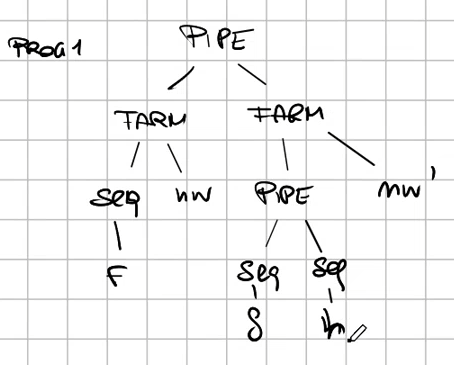
\includegraphics[scale=0.5]{34.png}
\end{center}
\textbf{Refactoring} or rewriting means looking at the semantic of the pattern and recognize shapes with the same \textbf{functional semantics} (\textit{what} is being computed) but different \textbf{non-functional semantics} (\textit{how} it is being computed, meaning different parallelism degrees or ordering of computation).
\subsection{Refactoring Rules}
\begin{list}{}{}
	\item Farm($x, n$) $\equiv$ Farm($x, m$) with $m\neq n$ (\textbf{pardegree change})
	\item Pipe($x, y$) $\equiv$ Comp($x, y$) (\textbf{pipe intro/elim})
	\item Pipe(Farm($x, \:$), Farm($y, \:$)) $\equiv$ Farm(Pipe($x, y$),$\:$)
	\item $x \equiv$ Farm($x$) (\textbf{farm intro/elim})
	\item Map(Comp($x, y$)) $\equiv$ Comp(Map($x,y$)) (\textbf{map fusion})
	\item \ldots
\end{list}
The questions revolve around choosing the best one. This is a \textbf{space exploration problem}: starting with the original tree $t_0$, using the refactoring rules we produce a number of derived trees and for each we measure a goal function (e.g. service time, so $T_{S0}$ for $t_0$). We move toward the best one, and repeat. So we do not explore the whole tree of derived graphs, but just the sub level of the current best graph. This greedy path should bring to a better solution, a better graph thus a better pattern for the current problem. This is \textbf{not possible}. Let's see why with a counterexample, e.g. Pipe(Seq($f$), Farm(Seq($g$), Seq($h$)) with $T_{S0}$ and show a way to reach a better $T_S$ with intermediate steps that have a worse $T_S$.
\begin{center}
	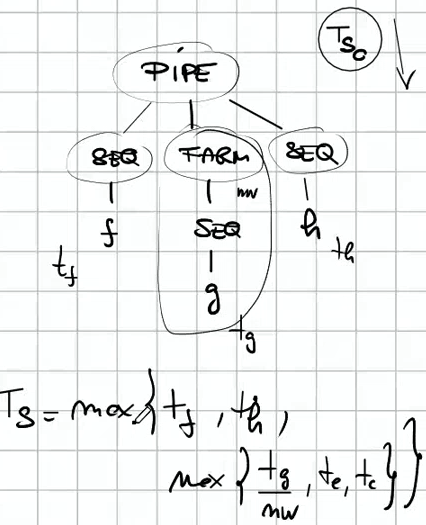
\includegraphics[scale=0.5]{35.png}
	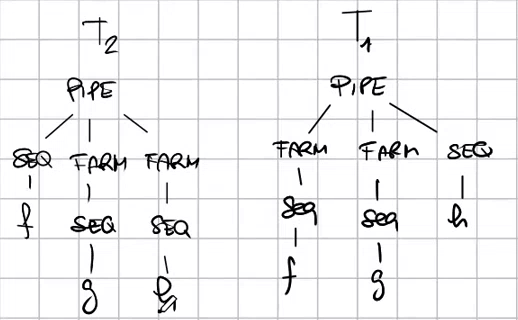
\includegraphics[scale=0.75]{36.png}\\
	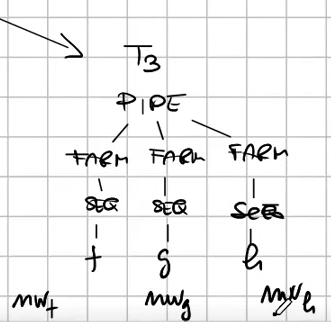
\includegraphics[scale=0.75]{37.png}
\end{center}
Each of these steps lowers the $T_S$: e.g. we imagine a bottleneck on one stage and introduce a farm there, then a bottleneck on the remaining stage and introduce another farm ending in $t_3$. But let's see another possible path: starting from $t_0$, in $t_4$ we remove the farm in the second stage, ending with Pipe(Seq, Seq, Seq). This would increase $T_S$. Then in $t_5$ we remove the pipeline, ending with Comp(Seq, Seq, Seq), once again increasing $T_S$. In $t_5$ we introduce a farm making Farm(Comp(Seq, Seq, Seq)) and here we can decrease $T_S$ as much as we want by increasing the parallelism degree, up to $T_S=\max\{T_{\hbox{scheduler}}, \frac{T_w}{nw}, T_{\hbox{collector}}\}$ with $T_w = t_f+t_g+t_h$ in our case, so with a $nw$ such that the maximum becomes either the time required by the scheduler or the collector.\\\\
So by performing a greedy search we easily fall into local minima, and thus we have to generate as much configuration as possible. So taken a certain tree $t_0$, using the rules we get all trees with depth $< k$ and then we apply map($T_S$) followed by a reduce($\min$) (or reduce($\max$) depending on what we want in place of $T_S$).
\subsection{Normal Form}
Speaking about stream parallel computations. Earlier we saw how the best pattern for the example was Farm(Comp(Seq, Seq, Seq)). \textbf{This pattern is optimal with respect to the $T_S$} taking in account the resources (same or smaller $T_S$ using the same or fewer resources).\\
Given a tree composed only by stream parallel patterns:
\begin{enumerate}
	\item Get the \textbf{frontier}, which is the \textbf{set of the sequential leafs}, \textbf{from left to right}.
	\item Compose the frontier \textbf{Comp(frontier)}
	\item Farm it out \textbf{Farm(}Comp(frontier)\textbf{)}
\end{enumerate}
This \textbf{always optimizes} the stream parallel computation in \textbf{stateless} situation. The principle is to transform a set of small computations spread around and put them into a big chunk of code with an input and on output, so \textbf{increase the grain of the computation}. The \textbf{grain} is \textbf{the ration between time spent computing and time spent organizing the computation}.
\subsection{Performance Model Usage}
Performance models are used in two ways:
\begin{list}{}{}
	\item \textbf{Evaluate} a certain value, e.g. $T_S$, by visiting the tree from leafs to root and computing the required value.
	\item \textbf{Optimize} by figuring out the parameters, e.g. $nw$
\end{list}
\subsection{Optimization}
In RPLSH we can do \texttt{optimize main with max resources}.
\section{Load Balancing} Giving the same amount of work to all the cores involved. Even if a single thread takes longer than all the other, we wait that it fishes so we have a lot of empty time in the other threads. The efficiency lowers a lot, and poor speedup too.\\
One of the reasons could be that the computation per se is unbalanced.
\subsection{Static Techniques}
Related to the usage of different splitting policies.
\paragraph{Chunk policy} Take the vector and split into adjacent parts
\paragraph{Cyclic policy} First item to first thread, second to second thread\ldots e.g. with two threads: first to th1, second to th2, third to th1, fourth to th2\ldots
\paragraph{Mix} A cyclic distribution of blocks. Split into blocks and assign the first to a thread, the second to the next\ldots following the cyclic policy.
\subsection{Dynamic Techniques}
We can do much more, adapting to the situation giving more things to do to the thread that so far have done less.
\paragraph{Autoscheduling} Threads are not assigned a block/item or a distribution, but each threads \textit{asks} for something to be computed. Some code like \begin{lstlisting}
while (more work to do) {
	ask work
	compute
	deliver result
}
\end{lstlisting}
The threads that gets longer tasks stops asking for more tasks for a while, and more tasks will be executed by the other threads. When tasks are almost finished, it may happen that some thread gets the "last" long task still taking longer than all the other threads. But it's not as impactful as stated before, as it's the worst case.\\
In general, prefetch $k \simeq 2$ or $3$ tasks
\paragraph{Job Stealing} Bunch of tasks, cyclic static assignment. With $nw$ threads and $m$ tasks, each thread gets $\frac{m}{nw}$ tasks. With job stealing, the thread that has finished its tasks and perceives that there's more to compute, steals a task from another thread. Problems: "size" of the steal, synchronize accesses, who to target\ldots the solution is a random policy: threads that finishes their own assigned task steal a random number $\in[0, nw]$ and steal that number of tasks.
\paragraph{Autoscheduling + variable size chunks}

\paragraph{Template Based Implementation} For each pattern (pipe, farm, map, stencil\ldots) we have templates:\begin{list}{}{}
	\item for each target architecture (multicore, cloud\ldots)
	\item activity graph
	\item performance modelling, also a way to have an idea of what we can achieve in terms of perfomance
\end{list}
Let's analyze a template for a pipeline on a shared memory multicore machine (\texttt{template(pipeline, SMmulticore)}):
$$\longrightarrow\hbox{thread}\rightarrow\hbox{thread}\rightarrow\ldots\rightarrow\hbox{thread}\longrightarrow$$
With the $\rightarrow$ being communication channels (queues). Modelling the speedup$(m)\simeq m$ with $m$ being the number of stages, so a linear speedup, if and only if $\max\{t_i\}\simeq t_j$ so the times of each stage are more or less the same.\\\\
But we can have another template
$$x_m\ldots x_2\:x_1\longrightarrow\hbox{queue}$$
Where in the queue we put "\texttt{compute} $f$ \texttt{over} $x_i$" as $\langle f,x_i\rangle$ for each $i$. Each worker gets $\langle f,x\rangle$ and puts in the queue $\langle g, f(x)\rangle$. For $\langle g,x\rangle$ returns $\langle h,g(x)\rangle$ and for $\langle h,x\rangle$ returns $\langle$ end$,h(x)\rangle$.\\
So the queue will have different types of tasks: the input tasks are assigned to $f$ but the intermediate tasks are assigned to $g$ or $h$: it's a pipeline. Of course, the end tasks means outputting on the output queue.\\
A problem: the queue is a bottleneck. We can use some techniques: set of queues, local queues\ldots Also the ordering, but i can keep the index $i$ for each stage and use it at the end to keep in a buffer and output in the correct order.\\
With modeling provided sufficient $T_A$, the speedup can be proportional to $nw$ and not $m$.\\\\
Another template is a round-robin scheduler that assigns to some workers that deliver results to sorter with respect to the input order. The scheduler gives $\langle i, x_i\rangle$ and the output is $h(g(f(x_i)))$ ordered on $i$. Pipeline. Uses $nw+2$ concurrent activities, with a queue for each worker plus a queue for the sorter. With $T_A$ low, we have speedup circa $nw$.\\\\
Changing architecture, from shared memory multicore to a clustered workstation. I can use any template ported to a cluster. For example
$$\hbox{workstation}_1\rightarrow_{\hbox{TCP/IP}}\hbox{workstation}_2\ldots$$
The speedup is circa the number of stages. But we can also have a number of workers in each workstation, with a scheduler and a merger per each. A kind of composed template, the third inside the stages of the first.
$$T_S\simeq\frac{\max\{T_i\}_{nw}}{nw}$$
The overhead is in the scheduling and merging parts of each stage. The scheduling is necessary, but in the ordering part we sort data on the input order, but we can do that just at the end of the last stage.
\paragraph{Macro Data Flow Implementation} With Data Flow we denote the operations where the order of computations are dictated by the flow of data encountered by the program counter.\\
So we have nodes that are composed of $\langle$ operator, variables, output$\langle$. For example, $$(a+b)\cdot(c-d)$$ can be represented as 
\begin{center}
	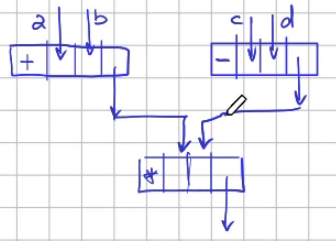
\includegraphics[scale=0.5]{7.png}
\end{center}
We have tokens on the inputs, that represent when data are available. When all data is available, the node becomes "fireable". This technique can be used to implement parallel patterns, Macro because instead of considering operations as nodes with functions an input/output nodes we consider macros with full portions of code instead of primitive functions.\\
Let's consider a program \texttt{main.cpp} that uses some pattern internally from a pattern library. First step: from a pattern tree we compile the MDF (Macro Data Flow graph). We have a graph repository and a pool of executors: anytime I have some input data I create a copy of the graph in the repository with the tokens that represent the data.\begin{center}
	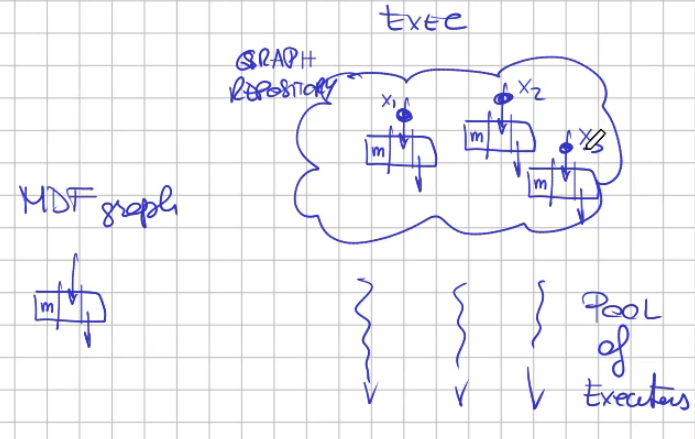
\includegraphics[scale=0.5]{8.png}
\end{center}
Each executor executes a loop where they get a fireable instruction, compute and deliver the output tokens.
\paragraph{Compiler} From the Pattern Tree it outputs the MDF graph.
\begin{list}{}{}
	\item Compile(Pipe($f,g$)) $\rightarrow$ $\langle f,$ in, A$\rangle$, $\langle g,$ A, out$\rangle$
	\item Compile(Seq($f$)) $\rightarrow$ $\langle f,$ in, out$\rangle$
	\item Compile(Farm($f$)) $\rightarrow$ Compile($f$) for each instance of input
	\item Compile(Map($f$)) $\rightarrow$ Compile($f$) for each element of the input collection
	\begin{center}
		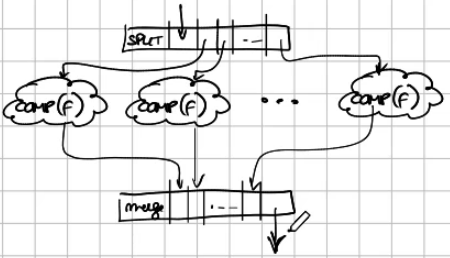
\includegraphics[scale=0.5]{9.png}
	\end{center}
	\item Compile(Reduce($f$)) $\rightarrow$ \begin{center}
		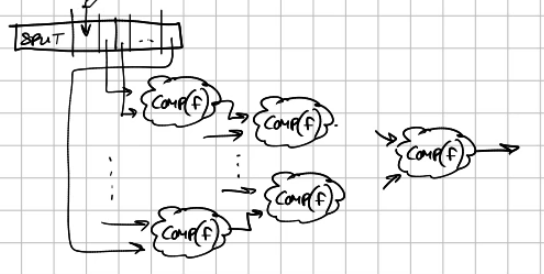
\includegraphics[scale=0.5]{10.png}
	\end{center}
\end{list}
Each one of the graphs has one input token and one output token, mandatory to be able to compose the graph. The Farm parallelism disappears %TODO
and third %TODO
\paragraph{Problems}\begin{list}{}{}
	\item Contention over repository
	\item Token delivery
	\item Maintain the list of fireable instructions
	\item Reordering on the out stream
\end{list}
\paragraph{Refactoring Rules}
The grammar used to write our program is:
\begin{center}
	Pat = Seq() $|$ Pipe(Pat$_1$, Pat$_2$) $|$ Comp(Pat$_1$, Pat$_2$) $|$ Farm(Pat, $nw$) $|$ Map(Pat) $|$ Reduce(Map)\\
	Prog $\Rightarrow$ Pat : $x$\\
	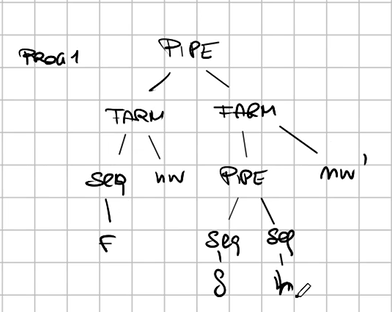
\includegraphics[scale=0.5]{12.png}
\end{center}
Whit \textbf{functional semantics} we mean \textbf{what is computed}. \textbf{Non-functional semantics} refers to \textbf{how} the result \textbf{is computed}.\\
So refactoring rules describe the equivalences in the \textbf{functional semantics}. So different performance, parallelism degrees\ldots\\
Some examples:
\begin{list}{}{}
	\item Farm($x, n$) $\equiv$ Farm($x, m$) with $n\neq m$
	\item Pipe($x, y$) $\equiv$ Comp($x, y$)
	\item Pipe(Farm($x, \_$), Farm($y, \_$)) $\equiv$ Farm(Pipe($x, y$) \_)
\end{list}
How to figure out the better ones? We will consider a small set of rules:
\begin{list}{}{}
	\item \textbf{Pipe introduction/elimination}: Comp($x,y$) $\equiv$ Pipe($x,y$)
	\item \textbf{Farm introduction/elimination}: $x \equiv$ Farm$(x)$
	\item \textbf{Map fusion}: Map(Comp($x,y$)) $\equiv$ Comp(Map($x,y$))
	\item \textbf{Pardegree change}: Farm($x, n$) $\equiv$ Farm($x, m$) with $n\neq m$
\end{list}
The idea is to write a program (so a tree $T_0$) and apply the rules (via a tool) getting $T_1,T_2,\ldots$ all functionally equivalent to $T_0$. Usually the goal is a low $T_{S_i}$. We take the produced trees, mapping each to its $T_S$ and reducing to $\min$ to get the minimum $T_{S_k}$.\\
But maybe we compute worse trees. I can do another thing: taking $T_0$ trying to find the path in the possible trees. I apply rules and measure the metric (in this example, $T_S$). Then I don't go exploring all the subtrees, applying all applicable rules, but I just go one level down and pick the best one each time. We follow a path that always gives a better (or equivalent) performing solution. But this is \textbf{not possible}.
%TODO why, 2nd part 22/03
With a lot of approximations and details ignored, I can figure out the best parallel architecture.
\paragraph{Normal Form} Speaking of stream parallel computations. Optimizes the service time $T_S$ (more precisely, the throughput).\\
We can derive the normal form from every pattern tree, only with stream parallel patterns\begin{enumerate}
	\item \textbf{Get the frontier}, set of all the sequential leaves in the tree, \textbf{left to right}.
	\item Comp(frontier), so sequential composition in the order they appear.
	\item Farm(Comp(frontier))
\end{enumerate}
This process always aims at optimizing the parallel computation. Unless there are some particular reasons. We take the whole set of things to compute an put them together (1 and 2), meaning creating a chunk of code that do the work: \textbf{increase the grain of the computation}.\\
This optimizes the service time taking also into account resources.
\paragraph{Performance Models} Used to evaluate or to optimize.\\
\textbf{Evaluate} meaning that, having a tree, we evaluate a metric (e.g. $T_S$) visiting the tree from the leaves. For each leaf we're interested in the sequential time ($T_S = L$ for the sequential nodes). The we go up one step visiting the parents: we have the parameters of the subtree and can compute $T_S$ of the node given its subtrees. We can repeat until the root.\\\
The visit of a tree is also a pattern, so if I take that pattern (visiting a tree from the leaves upward) passing the tree as a parameter I can get a number of different \textbf{visitors}: $T_S$ in this case is a visitor. For example, for Visitor(\# resources) we would visit the tree in the same way but using a different formula for computing the contribution of each node.\\
\textbf{Optimize} the parameters, for example the parallel degrees of the stages. In \texttt{rplsh} we used \texttt{optimize main with max resources}. How it's implemented? We take the tree, with Pipe in the root, same as before. We turn the tree with the $nw$ figured out, but we have a certain number of resources. For example we want to shrink the number of resources to match the number of cores.
\paragraph{RPLShell} \begin{center}
	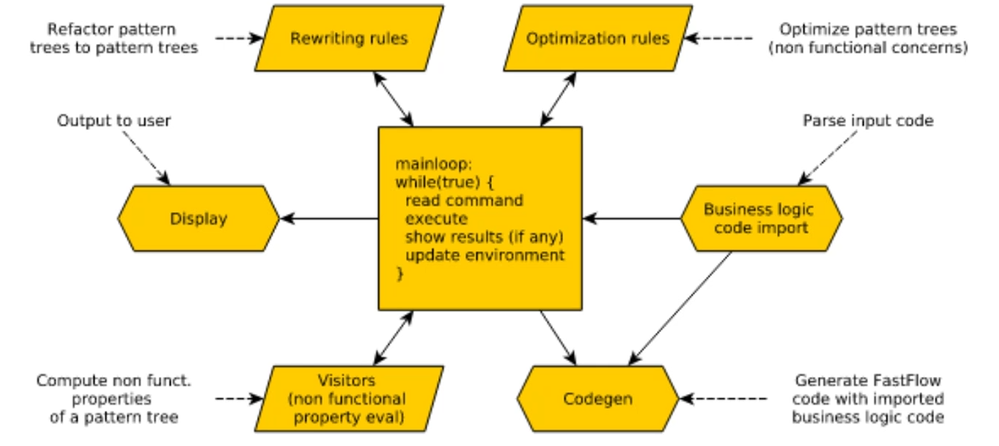
\includegraphics[scale=0.5]{13.png}
\end{center}
\begin{list}{}{}
	\item \textbf{Rewriting Rules} are the set of factoring rules.\\
	For example, we have the facts that allow me to rewrite a given tree $t$ as Farm($t$) or Pipe($t_1,t_2$) as Comp($t_1,t_2$).
	\item \textbf{Optimiziation Rules} the set of rules that for example transform a Farm(Farm($w$)) into Farm($w$) (because two farms linked are bad for performance), known as farmfarmopt, or the farmopt that is used when we have Farm($w$) with a certain $T_S$ of the $w$ and a certain $T_S$ target of the farm in order to set the $nw$ of the farm to $\frac{T_S}{T_{S,w}}$.
	\item \textbf{Visitors} the elements that visit the tree upwards.
\end{list}
\paragraph{Autonomic Management of Non Functional Features} In long running computations.\\
For example the classical variations in network load between night and day. Autonomic because %TODO
Born from industrial processes management, changing behaviors of the systems. Different architectures of the controller:
\begin{list}{}{}
	\item \textbf{MAPE Loop} (Monitor, Analyze, Plan, Execute loop)\\
	Execute activities via actuators, and the system has a set of actuator objects that can be invoked to change the behavior of the system (for instance changing $nw$). The system has sensors, too, that provide data to the monitor part.
\end{list}
We have to devise a strategy to be used. E.g.: if $T_A$ drops, most likely I could just increase $nw$ and viceversa if $T_A$ increases I can drop $nw$. Being more clever: let's suppose that $T_A$ goes from $T_{A_{\max}}$ to $T_{A_{\min}}$ in a $\sin$ fashion, when I'm in the minimum I could take time in taking a decision to increase $nw$ while $T_A$ is already increasing. Same for the maximum, I could spend time making the decision and always arriving late. So our strategy can be update: I can observe the changes and avoid situations of alternating opposite changes (in the example, the adding and taking away workers constantly).\\\\
To implement these strategies, I need \textbf{sensors} and \textbf{actuators}.\\
We need to observe the interarrival time $T_A$. Also need a data structure to observe the changes, by doesn't require sensors. These sensors would be in the emitter thread.\\
We need to increase or decrease $nw$, so the actuators must be able to achieve that. To add a worker, e.g. a thread, we need to know the queue for that worker, the collector\ldots so the emitter sounds like a good place.\\\\
This is implemented in the \textbf{control program} of our manager. Very crude \texttt{if (condition) do actuator;}.
\paragraph{ECA Rules} Set of \textbf{Event, Condition, Action} rules implemented in a rule system (e.g. \texttt{jboss}).\begin{list}{}{}
	\item \textbf{Event}: \textbf{triggering action}, e.g. $T_A$ change.\\
	Not the event per se to be taken into account.
	\item \textbf{Condition}: \textbf{predicates} on monitored values, internal state and events, that state whenever this particular rule has to be fired or not.
	\item \textbf{Action}: \textbf{set of actions} on the system or the state that must be \textbf{executed after some triggering event when the condition holds true}.
\end{list}
\subparagraph{Example}
\begin{center}
	\begin{tabular}{c | c c c}
	& \textbf{Event} & \textbf{Condition} & \textbf{Action}\\
	\hline
	$R_1$ & Change $T_A$ & \makecell{Less than the\\previous one} & Adding a worker\\\\
	$R_2$ & Change $T_A$ & \makecell{More than the\\previous one} & Removing a worker\\\\
	$R_3$ & Change $T_A$ & \makecell{Less than the\\previous one AND\\$nw$ just decreased} & \texttt{nop}, update $T_A$\\\\
	$R_4$ & Change $T_A$ & \makecell{More than the\\previous one AND\\$nw$ just increased} & \texttt{nop}, update $T_A$
	\end{tabular}
\end{center}
\paragraph{Contracts}\begin{enumerate} %TODO
	\item Propagate the "contract" top-down and try to implement it "best-effort"
	\item Manage to keep contracts satisfied 
\end{enumerate}
We're taking into accounts performance, but often power consumption is more important. These are both non-functional features. If we take into account both, we could implement a manager for each. But the managers may take decision that contrast with each other. A solution is to build a single manager that takes into account both features, into a single MAPE loop. But this requires that both knowledge are in a single place, bad for the separation of concerns. Another solution is to have two managers, one for each feature, each with its MAPE loop, and the two can communicate: the plan phase inform each other in the hope to have authorization for a change that the execute part needs, if we don't get the authorization we go for a \texttt{nop}.
\begin{center}
	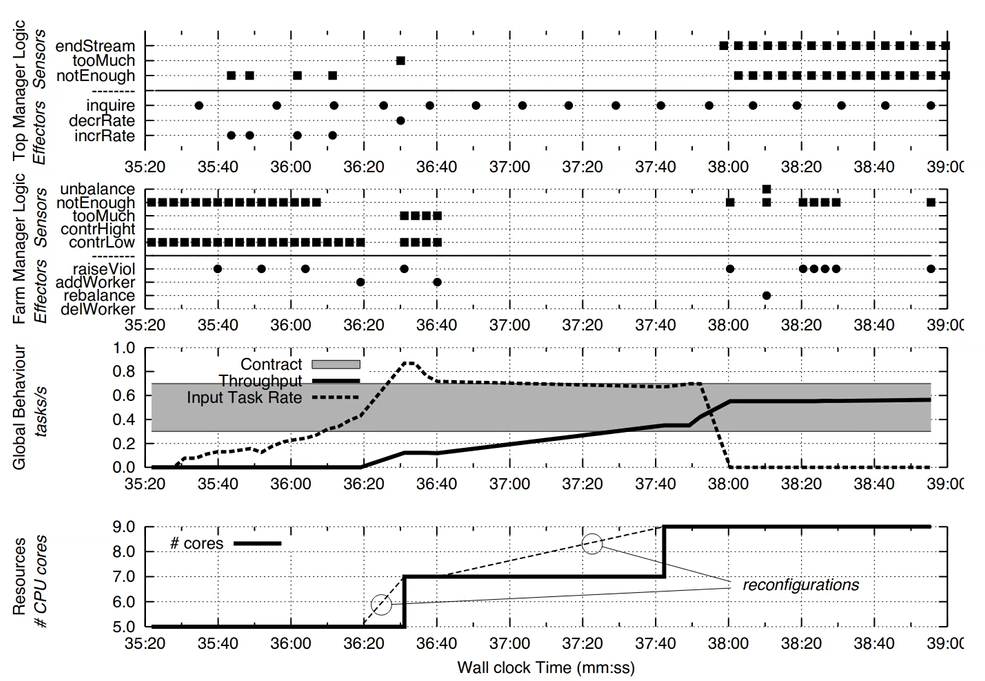
\includegraphics[scale=0.5]{15.png}
\end{center}
\section{Vectorization}
Very old technique. %TODO
Given $x, y, z$ as vectors of $x_i, y_i, z_i$ from $0$ to $n-1$ and $\forall\:i\in[0,n-1]\:\:z_i=f(x_i,y_i)$, implemented e.g. as a \texttt{for}. If the computation $f(x_i, y_i)$ is indepdendent of the other loop iterations (that is, $x_i$ is independent from all other $x_j, j\neq i$) then this is easily parallelized. A classical example is matrix multiplication: $$\forall\:i\:\:\forall\:j\:\:\forall\:k\:\:c_{ij} = a_{ik}\cdot b_{kj}$$
2 steps: we need to have zeroes in the first positions and %TODO
We have ways to load/store vectors to %TODO

Hardware designed specifically, vector processors. Registers that can be seen as vectors of tot bits numbers: 256 bits vector registers seen as 4 64 bits numbers, or 8 32 bits numbers and so on. With special commands, for example \texttt{VADD.I32 R1, R2, R3} meaning R1 = R2 + R3 with I32 meaning 32 bit numbers with I index.
\paragraph{Conditions} In \texttt{g++} we can explicitly ask with \texttt{-03 -ftree-vectorize} and with \texttt{-fopt-info-vec-[missed/all]} ask what cannot be vectorize.\\
The conditions are:
\begin{list}{}{}
	\item Need to know the number of iterations.\\
	\texttt{for} is ok, \texttt{while(c$<$k)} sometimes cannot be vectorized
	\item Cannot call external code in the loop body, functions or libraries.
	\item No conditional code.\\
	It'd require compiling two paths, so complicates things.
	\item No overlapping pointers.\\
	
\end{list}
\paragraph{\texttt{\#pragma}} Indications to the compiler\\
\texttt{\#pragma GCC ivdep} tells the compiler whatever it thinks of the loop, to consider it as independent iterations.\\
\texttt{\#pragma GCC unroll n} tells the compiler that the following loop should be unrolled \texttt{n} times. Useful for short loops.\\\\
So vectorization very useful for mathematical operations, such as differential equations. Requires to take a bit of care in the core to be able to vectorize. If we don't convince the compiler, we can use the \texttt{pragma}.\\
If we vectorize Farm($f,nw$), the speedup with the vectorized $f$ with respect to the non-vectorized $f$ is smaller. Because the vectorized code in general is faster, so non-vectorized Speedup($nw$) $Z$ Vectorized Speedup($nw$).\\
But vectorization can radically change the $T_S$ of the stages of a Farm, for instance, and introduce waiting times for workers. You don't change the sequential fraction, just the non-sequential fraction.
\paragraph{Libraries} Libraries include operations used often, e.g. \texttt{Blas} (basic linear algebra system) or \texttt{Lapack} or \texttt{NKL}.\\
For instance \texttt{blas} provides \texttt{gemm} for very optimized matrix multiplications.\\
Use libraries because they are very optimized, exploiting all the possible optimizations.
\paragraph{GRPPI} C++ library that implements common parallel patterns, using standard threads or other backends (e.g. omp, tdd or fastflow). The backend is only modeled by the \texttt{execution} parameter.
\section{OpenMP}
\paragraph{MPi} Directed to clusters and workstations, multicores
\paragraph{CDA/OpenCL} For GPU
\paragraph{OpenMP} Parallel for, targets shared memory multicores (and GPU/FPGA). Very dated, since 1997 the version 1.0: no GPU, even multicores were not very popular.\\
At the beginning very simple API that provided launching threads in parallel and something related to the parallel for. Each version improved on that, introducing: tasks, target accelerators, depend clauses on tasks (to tell that a task must be executed only after the completion of another task), memory management, task reduction (among values of different tasks), task affinity\ldots\\
When we speak about shared memory multicores, we speak of some situation where in the board we have more than one sockets with multicore in each socket.
\paragraph{Concepts}\begin{list}{}{}
	\item \textbf{Directives}, which OpenMP is based on. Directives, in C/C++ environment, are kind of pragmas which can be understood as portions of compiler
	\item OpenMP is \textbf{compiler-based}
	
\end{list}
As pros:
\begin{list}{}{}
	\item Few lines of code are required to run parallel code, opposed to writing all the logic by oneself
	\item Keep sequential code, means we can perform functional debugging and then adding parallel pragmas
\end{list}
As main con we need to rewrite the compiler, not entirely (such as the parser), but everything related to the usage of the pragmas must be generated at compile time.\\
E.g. the map seen in the GRPPI library is written at higher level but in the library, doesn't touch the compiler.\\\\
We have something used to \textbf{set up parallel activities} and something different used to \textbf{organize the parallel computation} using the parallel activities available.
\paragraph{\texttt{\#pragma omp parallel}} This must be placed before a statement, it tells the compiler that the following block must be executed in $nw$ copies (threads) if and only if $nw$ is the number of resources/cores of the current machine.\\
Most directives have clauses used to specify parameters. E.g. \texttt{num\_threads(nw)} tells to use the variable $nw$ instead of the predefined one (the number of cores).
\begin{lstlisting}[style=myC]
#include <iostream>
#include <omp.h>

using namespace std;
int main(int argc, char** argv) {
	int nw = 1;
	if (argc != 1)
		nw = atoi(argv[1]);
	#pragma omp parallel num_threads(nw) // clause
	{
		auto id = omp_get_thread_num();
		cout << "Ciao from id " << id << endl;
	}
	return(0);
}
\end{lstlisting}
\paragraph{\texttt{\#pragma omp single}} Specifies that the following statement/block is to be executed by just a single thread.
\begin{lstlisting}[style=myC]
#include <iostream>
#include <omp.h>

using namespace std;
int main(int argc, char** argv) {
	int nw = 1;
	if (argc != 1) {
		nw = atoi(argv[1]);
		#pragma omp parallel num_threads(nw)
		{
			#pragma single // this will be executed by a single thread, just one enters the following line, use a block for more lines
			cout << "Id " << omp_get_thread_num() << " of " << omp_get_num_threads() endl;
		}
	} else {
		#pragma omp parallel
		{
			auto id = omp_get_thread_num();
			cout << "Id " << id << " of " << omp_get_num_threads() endl;
		}
	}
	return(0);
}
\end{lstlisting}
\paragraph{\texttt{\#pragma omp critical}} To execute the next code in mutual exclusion.
\paragraph{To use OpenMP} Compile with flag \texttt{-openmp}.\\
The \texttt{a.out} compiled, when executed, uses the linked library which provides several things including a lock/mutex machanism. So instead of the \texttt{\#pragma omp critical} we can use \texttt{\#pragma omp parallel} and then just the lock/unlock:
\begin{lstlisting}[style=myC]
omp_lock_t lock;
omp_init_lock(&lock);
#pragma omp parallel
{
	// code
	omp_set_lock(&lock);
	// mutex code
	omp_unset_lock(&lock);
	// code
}
\end{lstlisting}
With the code/unlock declared with respect to the OpenMP library.
\paragraph{Different code for different threads} We can do something like
\begin{lstlisting}[style=myC]
#pragma omp parallel num_threads(2)
{
	if (omp_get_thread_num() == 0) {
		// code for thread 1
	} else {
		// code for thread 2
	}
}
\end{lstlisting}
This is \textbf{SPMD} code: single program multiple data.
\paragraph{Sections directive}
\begin{list}{}{}
	\item \texttt{\#pragma omp sections}: identifies a command which is filled by other \texttt{section} directives, each executed possibly in parallel
	\item \texttt{\#pragma omp section}
\end{list}
Example
\begin{lstlisting}[style=myC]
#pragma omp sections
{
	#pragma omp section
	{
		//code 1
	}
	#pragma omp section
	{
		//code 2
	}
}
\end{lstlisting}
All the \texttt{section} may happen in parallel, how much is defined and can be inherited by other statements. For example I can have a \texttt{\#pragma omp parallel} before the \texttt{\#pragma omp sections}, giving the threads explained before (the number of cores as default, or as specified by \texttt{num\_threads(nw)}.
\paragraph{Variables} In most directives you can append clauses that specifies the behavior of variables.\\
For example in parallel pragmas you can append the clauses\begin{list}{}{}
	\item\texttt{private(x)} (non initialized local copy local to each thread)
	\item\texttt{firstprivate(x, y)} (get a local copy initialized from previous value)
	\item\texttt{shared(y, z)} (inherit value from the global environment)
	\item\texttt{lastprivate(x)} (this one legal only in sections, not in parallel, local copy then last \texttt{section} copied to global environment, take care last one means in syntactic-fashion, the last syntactic section updating the variables copies to global environment)
\end{list}
\paragraph{\texttt{\#pragma omp for}} Most famous and used.\\
The default behavior is that the iterations, e.g. from $i=0$ to $i=n-1$, are made into $nw$ chunks given each to a thread. Obviously we need independent iterations. There are others scheduling policies, specified with clauses appended to the \texttt{\#pragma omp for}:
\begin{list}{}{}
	\item \texttt{static} the default one, with the option of specifying \texttt{chunksize(m)} specifying the number of items in each chunk, so $\frac{n-1}{m}$ chunks of $m$ items, given to the threads in a round-robin fashion
	\item \texttt{dynamic} where the threads ask for new chunks when they have finished, chunks are assigned on demand. Same of the static for other things
	\item \texttt{guided} use a number of chunks smaller and smaller: large chunks in the first part of the array, then smaller chunks, then smaller and so on. Intended to be used for unbalanced computations: at the beginning we assign large chunks to each thread, but the threads may finish at different times and get smaller chunks to accomodate for load unbalancing
	\item \texttt{auto} everything decided by the compiler
	\item \texttt{runtime} keyword which inherits the scheduling policy from an environment variable which has to be defined before 
\end{list}
You also have other clauses
\begin{list}{}{}
	\item \texttt{nowait}, removes the implicit barrier to wait all the threads, present in the parallel pragma
	\item \texttt{reduction([+,*,and,or], x)}
\end{list}
\paragraph{\texttt{\#pragma omp task}} Kind of async, suggestion that if there are unusued threads use to compute the task otherwise it's sequential code.\\
Can define taskgroups to execute in parallel and wait with the implicit barrier at the end.\\
You can append \texttt{tied} or \texttt{untied}: with the first anytime you assign/reassign the execution of this task then it would be on the same thread.\\
The taskloop provides something similar to a map, or a pragma for, but subjecting to the rules of the tasks: could be executed in parallel given enough resources ecc.
\paragraph{Example} Sum of a vector with a reduce(+), base case being a vector of length 1 so return the value v[0]. Otherwise the recursive case is a vector of $n$ positions: compute the half and split in v[0,$\frac{n}{2}$] and v[$\frac{n}{2},n$] recur. So we need a task for the left half, a task for the right part, checking not to be in the base case.
\begin{lstlisting}[style=myC]
int sum (int* restricted v, int start, int end) {
	auto size = end - start;
	auto mid = size/2;
	int x, y; //shared for the subtasks, sum from left and right
	
	if (size == 1) return v[start]; //base case
	
	#pragma omp task shared(x) //to share the result with this "main" thread
	{
		x = sum(v, start, start+mid);
	}
	#pragma omp task shared(y) //same as befor
	{
		y = sum(v, end-mid, end);
	}
	#pragma omp taskwait //wait for the termination of the tasks, a "barrier"
	//now both tasks have finished, we have both x and y
	return x+y;
}

int main(int argc, char** argv) {
	#pragma omp parallel num_threads(nw) //or from the CLI "export OMP_NUM_THREADS=nw"
	//...
	#pragma omp single //single or master
	sum(v, 0, n-1);
}
\end{lstlisting}
\paragraph{Timing routines} Also present.
\paragraph{Taskpool} The idea is to set up $nw$ threads to execute tasks without awaiting any kind of results from the tasks. Some king of \texttt{void} function.\\
We can use \texttt{auto out = bind(function, parameter);}, with \texttt{void function(float x);},\\
then \texttt{out} will be a \texttt{function<float()>} so we can call \texttt{out();} because the parameter is already given.
\section{FastFlow}
Addresses the idea of structured parallel programming targeting shared-memory multicores. It's a open-source header only library (\texttt{-03 std=c++17}). It's a complete layered system:\begin{list}{}{}
	\item Parallel Applications
	\item \begin{list}{}{}
		\item High level parallel patterns
		\item Parallel building blocks (pipeline\ldots), and also a small library of transformers (to change shape of structures such as pipelines\ldots)
		\item Core library of FastFlow: sequential building blocks
	\end{list}
	\item Posix threads, RDMA libraries, OpenCL/CUDA
	\item HW layer: multicore shared-memory, but also GPU and FPGA accelerators, also COW (cluster of workstations) with TCP/IP and MPI
\end{list}
\begin{center}
	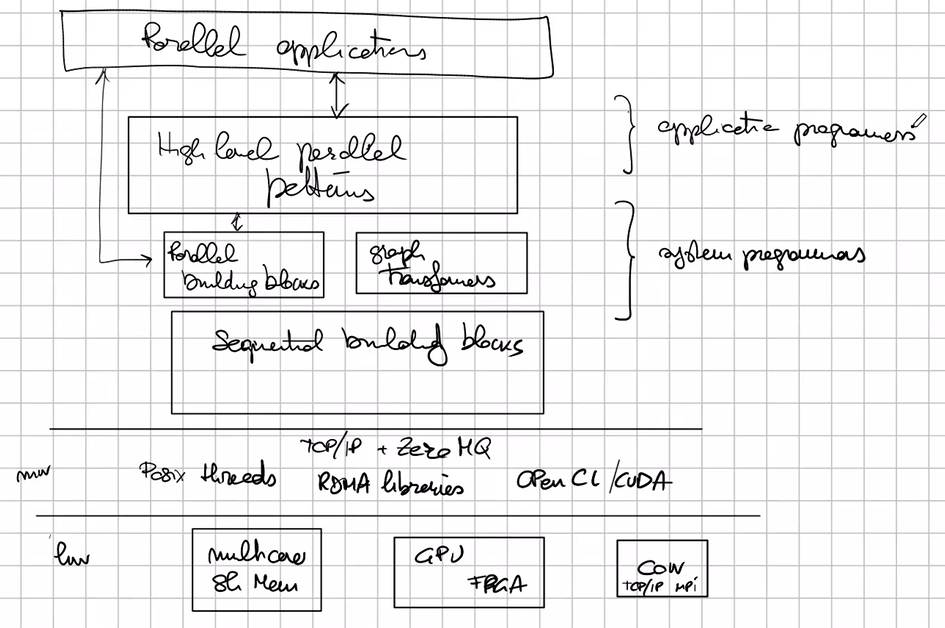
\includegraphics[scale=0.5]{16.png}
\end{center}
\paragraph{\texttt{ff\_node}} Computes some function and has two queues: a queue from where it takes items to be computed and a delivery queue.\\
FastFlow has stream computations and data-parallel computations.\\
Two nodes can be merged in a \texttt{pipe ff\_node}: this merges the output queue of the first node into the input queue of the second node.\\
The single nodes implement the business logic, the rest is managed by the framework.\\
In the \texttt{svc} method, being \texttt{void*} both in parameters and in return type, you can specify whichever type you need to flow through the tasks. You can pass a task as parameter, process it and cast to \texttt{void*} its result to return it. With \texttt{ff\_node\_t<t1, t2>} it's introduced the type checking at template level.
\paragraph{Stream} \begin{center}
	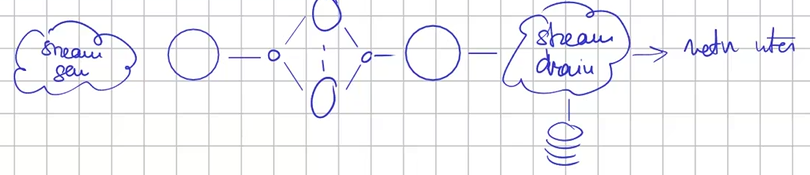
\includegraphics[scale=0.5]{17.png}
\end{center}
The stream flows through the program and it could be infinite, in principle. We have the interarrival time to consider, so we cannot look the entire stream as a whole data structures, at most you can see a certain window.
\begin{list}{}{}
	\item EOS, End Of Stream: value that signify that the stream has ended. Can be used as a condition to end loops (much like EOF for files)
	\item \texttt{ff\_send\_out} sends items in the stream. E.g. to end the stream, \texttt{ff\_send\_out(EOS)}
\end{list}
Shared-memory multicore, so each activity is a thread basically.\\\\
In the queues we host pointers, we don't move data. We target the fastest communication possible, non-blocking channels (without condition variables and other mechanisms): the native FastFlow queues has latency of less than tens of nanoseconds, due to cache overhead. But there are other channels, e.g.: the emitter for a farm is a 1:$n$ communication channel so we use a father thread, slowing down the process but it's inevitable. This can be changed at compile time to use blocking communication channels (structures with mutexes, variables\ldots).
\paragraph{\texttt{ff\_node\_t<tin, tout>}} Requires the type of the input and of the output. Requires to implement a methods\begin{list}{}{}
	\item \texttt{tout* svc(tin* task);} the body, the function computed by the thread.\\
	Has to \texttt{return(tout*)}, or a \texttt{return(EOS)} when it wants to end (passing to \texttt{svc\_end}, or a \texttt{return(GO\_ON)} that tells the framework that you finished the work but doesn't put anything in the output stream. Kinda like a "\texttt{skip} and give me the next item").
\end{list}
Other two method are optional, provided empty but can be rewritten:
\begin{list}{}{}
	\item \texttt{int svc\_init();} to initialize data before the computation, executed before \texttt{svc} over the input stream, e.g. to open a file
	\item \texttt{void svc\_end();} executed at the end, e.g. to close the file
\end{list}
\texttt{svc} stands for service.
\paragraph{Lifecycle of \texttt{ff\_node\_t}}\begin{enumerate}
	\item \texttt{svc\_init} called once when the thread is started
	\item \texttt{svc} called for each item appearing on the input stream\\
	Returns\begin{list}{}{}
		\item \texttt{tout*}
		\item \texttt{EOF}
		\item \texttt{GO\_ON}
		\item Other special values
	\end{list}
	\item \texttt{svc\_end} called right before terminating the thread
	\item \texttt{EOSnotify()} callback upon receiving \texttt{EOS}, to do something when it receives \texttt{EOS} because upon receiving that we don't call \texttt{svc} but go to \texttt{EOSnotify()} and then \texttt{svc\_end}
\end{enumerate}
\paragraph{Definition of the program} I can declare several \texttt{ff\_node\_t}\begin{list}{}{}
	\item \texttt{ff\_node\_t<vector<float>> t1;}
	\item \texttt{ff\_node\_t<vector<float>> t2;}
	\item \ldots
\end{list}
Then we can put in a pipeline
\begin{list}{}{}
	\item \texttt{ff\_Pipe p(t1, t2);}
\end{list}
So far no execution, only declaration
\paragraph{Running} We call the \texttt{run\_and\_wait\_end()} method, for example \texttt{p.run\_and\_wait\_end();} which starts everything.
\begin{lstlisting}[style=myC]
ff_node_t<vector<float>> t1;
ff_node_t<vector<float>> t2;
ff_Pipe p(t1, t2);

{
	utimer to("program");  // to time the execution
	p.run_and_wait_end();
}

\end{lstlisting}
\paragraph{Typical Patterns} With capital letter are higher level, the lower letter are lower level patterns \begin{list}{}{}
	\item \texttt{ff\_Farm(ff\_node\_t worker, int nw);} build a farm with $nw$ parallel degree of \texttt{worker}s as nodes
	\item \texttt{ff\_Pipe(ff\_node\_t stage, ...);}
\end{list}
\pagebreak
\begin{lstlisting}[style=myC]
#include <ff/ff.hpp>

struct source : ff_node_t<myTask> {
	myTask* svc(myTask* t) {  // source started with null as parameter, so t can be omitted
		for(int i = 0; i < N; i++) {
			ff_send_out(new myTask(i, ...));  // whatever you need to output
		}
		return(EOS);
	}
};

struct sink : ff_node_t<myTask> {
	myTask* svc(myTask* task) {
		cout << task << endl;
		return(GO_ON);  // processed and ready for next
	}
};

struct f : ff_node_t<myTask> {
	myTask* svc(myTask* task) {
		fun(t);  // e.g. it works by side effects
		return(t);  // whatever the process I need
	}
};

int main(int argc, char* argv[]) {
	// declaration
	source node1;
	f node2;
	sink node3;
	ff_Pipe<> pipeline(node1, node2, node3);
	// implies 3 threads, one for each node (parallelism degree = 3)
	
	
	// execution
	pipeline.run_and_wait_end();
	return 0;
}
\end{lstlisting}
Compile with at least \texttt{-03 -pthread}. This way uses non-blocking queues.
\paragraph{Pipeline} \texttt{ff\_Pipe<> pipeline(...);}
\paragraph{Usage statistics} Use \texttt{-DTRACE\_FASTFLOW} for debugging purposes, for usage statistics.
\paragraph{Creating tasks} For example a vector of \texttt{ff\_node} pointers, with \texttt{vecto<unique\_ptr<ff\_node>> W;}.\\
The \texttt{unique\_ptr} is an abstraction provided by C++ to associate a usage counter to a pointer, allocated by the system.\\
We then add the workers to the vector with \texttt{W.push\_back(make\_unique<funstageF>());}.
\pagebreak
\begin{lstlisting}[style=myC]
float fun(float x) {
	this_thread::sleep_for(2*tf);
	return x/2.0 + 1.5;
}

struct funstageF : ff_node_t<myTask> {
	myTask* svc(myTask* task) {
		task->x = fun(task->x);
		return task;
	}
}

int main(int argc, char* argv[]) {
	int m = atoi(argv[1]);
	int d = atoi(argv[2]);
	source s1(m, d);
	
	vector<unique_ptr<ff_node>> W;
	for (int i = 0; i < 5; i++) {
		W.push_back(make_unique<funstageF>());
	}
	cout << "Worker N. " << W.size() << endl;
	ff_Farm<myTask> f2(move(W));
	sing s4;
	
	ff_Pipe<> myPipe(s1, f2, s4);
	myPipe.run_and_wait_end();
	myPipe.ffStats(cout);  // compile with -DTRACE_FASTFLOW
	
	return 0;
}
\end{lstlisting}
\paragraph{Other types of nodes} You can use \textbf{Multiple Output nodes} \texttt{ff\_monode\_t} and \textbf{Multiple Input nodes} \texttt{ff\_minode\_t}.\\
In a classical \texttt{ff\_node\_t} you may just \texttt{return(something)} or \texttt{ff\_send\_out(something)} something that goes in the output queue.\\
In the multiple output node you can use \texttt{ff\_send\_out\_to(something, worker)} where you specify which worker may receive the data.\\
In the multiple input node you can use \texttt{ff\_get\_channel\_id()} used to understand which channel provided the result. You also have \texttt{from\_input()} that can be used to distinguish that type of channel (feedback channel or not).
\paragraph{RoundRobin} The default policy is round robin.\\
If compiled with \texttt{-DFF\_BOUNDED\_BUFFER} and \texttt{-DDEFAULT\_BUFFER\_CAPACITY=k}, program wide the queues will be bounded to $k$ elements. When the emitter finds all the queues full, it simply waits, looking for empty spots in all the queues.
\paragraph{Scheduling} In a farm, there's the method \texttt{farm.set\_scheduling\_ondemand()}. It's not a true on demand, meaning that a worker without work asks the emitter for something. Instead, this forces the input buffers to be short, kind of on demand because the queues will empty faster and the emitter will fill them faster, a good approximation of the worker asking for a task without the need of a feedback channel from each worker to the emitter.
\paragraph{OFarm} \texttt{ff\_OFarm} has the same rules as the farm pattern but Ordered, meaning that the collector of this farm sorts the results.\\
Limitations: workers cannot change the length of the string (no \texttt{GO\_ON} or multiple \texttt{ff\_send\_out} upon receiving a task), and workers has to be sequential.
\paragraph{Master Worker Pattern} Master directs tasks to workers and receives results. Can be achieved with a \texttt{ff\_Farm} playing with the parameters: eliminate collector, wrap-around (feedback loop) the workers. The problem is that with the wrap-around we have to be careful in handling the feedback loops.\\
The master also needs to discern the results of the workers (from the feedback loop) from the queue of tasks it has to send out coming from its queue. So we call the first time when there are no tasks in the queue, getting NULL as task in, and start the tasks returning \texttt{GO\_ON}, then waits for the results from the feedback channel.
\begin{lstlisting}[style=myC]
TASK* svc(TASK* tin) {
	if (tin == NULL) { //first run, start tasks
		for (int i = 0; i < m; i++) {
			TASK* t = new TASK{i, ((float) rand())/((float) INT_MAX), (rand()%100)};
			ff_send_out(t);
		}
		return GO_ON;
	} else { // getting tasks from feedback channels
		std::cout << "Feedback " << tin->taskno << " " << tin->x << std::endl;
		sum += tin -> x
		m--;
		if (m == 0) return EOS;
		else return GO_ON;
	}
}
\end{lstlisting}
\paragraph{\texttt{ParallelFor}} Needs \texttt{\#include <ff/parallel\_for.hpp>} because it's a higher level pattern.
\begin{lstlisting}[style=myC]
#include <ff/parallel_for.hpp>

ParallelFor pf; //we'll see the parameters later

pf.parallel_for(0, // initial value of the iteration value, e.g. 0 if int i = 0
				n, // limit of the iteration value, e.g. n if i < n
				1, // step incremen, e.g. 1 if i++
				0, // chunk size
				[](const int i) { }, // lambda for the ith iteration
				nw); // parallel degree
\end{lstlisting}
For example:
\begin{lstlisting}[style=myC]
for (i = 0; i < n; i++) {
	v[i] = f(v[i]);
}
\end{lstlisting}
becomes
\begin{lstlisting}[style=myC]
pf.parallel_for(0, n, 1, 0,	[&](const int i) { v[i] = f(v[i]); }, nw);
\end{lstlisting}
Chunksize of 0 means that the vector in $nw$ blocks of equal size and each worker gets a contiguous chunk of $\simeq \#$iterations$/\#$workers (\textbf{static scheduling}). With a chunksize of $>0$, we have \textbf{dynamic scheduling} with task granularity equal to chunksize (meaning that the vector is divided into blocks of chunksize elements, dynamically means that a idle worker gets a chunk), and with chunksize $<0$ we have \textbf{static scheduling} with blocks of chunksize elements same as before.\\\\
With the \texttt{\#pragma omp for} we can append many clauses, e.g. \texttt{reduction(+:sum)} (with an operator followed by a variable in the parentheses). For instance, in the following code
\begin{lstlisting}[style=myC]
#pragma omp for reduction(+:sum)
for ( ) {
	sum += x[i];
}
\end{lstlisting}
the sum is managed in parallel exploiting the threads: each thread has its own \texttt{sum}$_i$ variable and each intermediate sum are summed together (because we specified $+$) when the parallel for finishes.\\
The \texttt{ParallelForReduce} supports the name of the variable and the lambda function to apply. An example: need to compute dot product between $a$ and $b$, so $\sum_i a_i\cdot b_i$. Usually would do (sequential code)
\begin{lstlisting}[style=myC]
int sum = 0;
for (i = 0; i < n; i++) {
	sum += a[i] * b[i];
}
\end{lstlisting}
With parallel for
\begin{lstlisting}[style=myC]
// variable, zero value to initialize, starting from, ending to, increment, chunk size, lambda, final lambda, parallel degree
pfr.parallel_reduce(sum, 0, 0, n, 1, 0,
					[&](const int i) {sum += a[i]*b[i];},
					[&](int &s, const int ps) {s += ps;},
					nw);
\end{lstlisting}
\texttt{ParallelFor} is a \textbf{data parallel} pattern. At the end of the for there's a barrier that waits for all the threads involved to finish.
\paragraph{Divide and Conquer Pattern} \texttt{ff\_DC(divide, combine, base, cond, input, outpu, nw)}
\begin{list}{}{}
	\item \texttt{divide} splits the input
	\item \texttt{combine} puts together partial results
	\item \texttt{base} function applied to short portions/single elements
	\item \texttt{cond} is a condition that tells if you are in a short portion/single element
	\item \texttt{input} and \texttt{output} are the input and output vectors
	\item \texttt{nw} is the parallel degree
\end{list}
\paragraph{Macro Data Flow Pattern} Used to describe custom patterns: use tags to specify nodes and dependencies. An example: compute the following graph
\begin{center}
	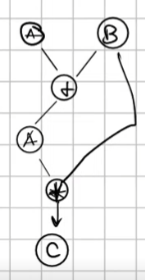
\includegraphics[scale=0.5]{21.png}
\end{center}
With a function that computes the sum \texttt{sum(a, b)} and one for the multiplication \texttt{mul(a, b)}. We setup some parameter info structures that tells the kind of usage of the parameters
\begin{lstlisting}[style=myC]
// A = A+B
param_info _1 = {&A, input};
param_info _2 = {&B, input};
param_info _3 = {&A, output};
// we've described that A and B are read and A is a result
// mdf is the Macro Data Flow object initialized before somewhere
mdf.add_task(P, sum, &A, &B, size); // append the node specifying the task
\end{lstlisting}
\paragraph{FastFlow Building Blocks} Few kind of blocks: sequential, parallel\ldots
\subparagraph{Sequential Building Blocks} Different kind based on number of inputs and number of outputs.
\begin{center}
	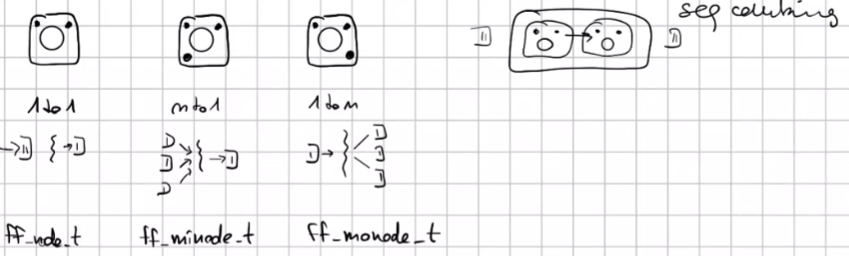
\includegraphics[scale=0.5]{22.png}
\end{center}
These can be combined sequentially.
\subparagraph{Parallel Building Blocks} Pipelines with: single block, two blocks, two blocks with a feedback channel of the second toward the first.\\
Farm style building blocks: emitter which connect to a set of nodes (workers), collector which takes from the workers. The emitter and collector are sequential building blocks that can be linked to parallel building blocks as workers.\\
All-to-all building blocks
\begin{center}
	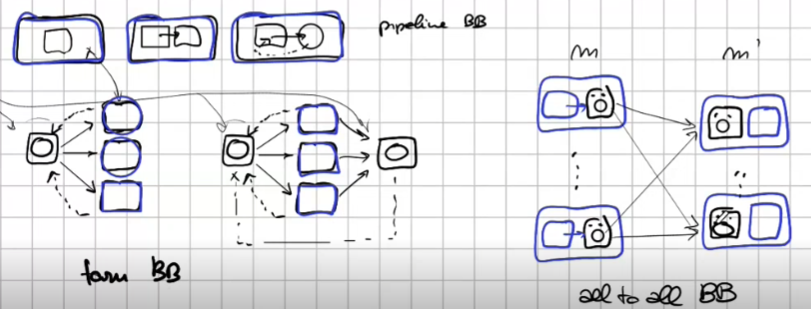
\includegraphics[scale=0.5]{23.png}
\end{center}
\subparagraph{Graph Transformers} For example having a Pipeline with a Farm as intermediate stage, meaning \texttt{ff.Pipe<int> mPipe(S1, Farm2, S3);}, we can optimize it including the sequential computation of the first stage S1 in the emitter of the Farm and the sequential computation of the last stage S3  in the collector of the Farm. We can declare a \texttt{optlevel opt;} optimizer and then set \texttt{opt.remove\_collector = true;}, \texttt{opt.merge\_with\_emitter = true;} and optimize with \texttt{optimize\_static(mPipe, opt);}. All this at declaration phase.
\paragraph{Concurrency Throttling} Useful to handle the pressure from the input, adding or removing workers accordingly. It's possible to declare a Farm with a given $nw$ and freeze some of the workers. Meaning that the emitter only perceives the non-frozen workers, the frozen workers are "ghosts" and may be unfrozen when needed.

\section{Parsec} Benchmarks %TODO lesson 28
\begin{list}{}{}
	\item \textbf{Blockslides} Portfolio of options, to compute the prices require partial differential equations
	\item \textbf{Cammeal}\\
	Simulated Annealing
	\item \textbf{Dedup}
	\item \textbf{Ferret} Pipeline
\end{list}
\begin{enumerate}
	\item Come up with an initial solution Pipe(S1, S2, S3, S4, S5)
	\item Refactoring techniques and possible explore the solution space to find the better solution\\
	Before coding! Insights on possible performance, possible solutions to discern the better one.
	\item Implementation phase of the better solution: OMP\ldots
\end{enumerate}
In the project, figure out from the sequential code the values of interest (e.g. time spent in the stages) and once we have a clear idea, refactoring and then implement the best solution.
\section{Stateful Computations} So far assumed that stateless stages/workers/components. E.g. in a Pipeline, the stages are functions $f,g,h,\ldots$ where we move $f(x)$ to $g$, $g(f(x))$ to $h$\ldots and we just compute function, no interaction between the stages.\\
In a stateful computation the computation depends on: input, state and the function. So not $f(x)$ but $f(x, state)$
\begin{center}
	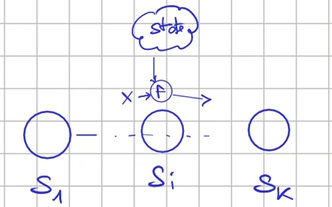
\includegraphics[scale=0.5]{18.png}
\end{center}
We don't mind the order of accesses in the state but it has to be accessed in mutual exclusion. If the accesses to the state happen at the same time, then it would be difficult to compute the times. So we make another assumption $t_i = t_{state_i} + t_{fun_i}$ with $t_{state_i}$ being the mutex.
\begin{center}
	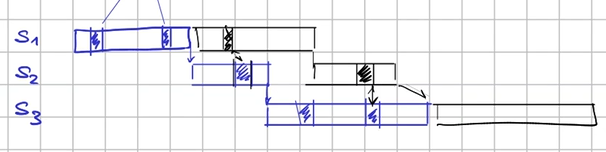
\includegraphics[scale=0.5]{19.png}\\
	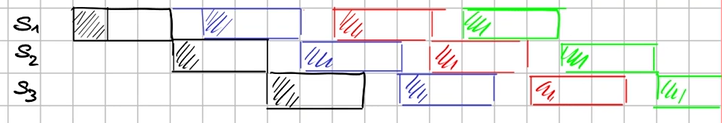
\includegraphics[scale=0.5]{20.png}
\end{center}
\paragraph{Accumulator} We have a parallel pattern and a \textbf{state pattern} (accumulator). Each parallel activity updates the pattern using a function $f$ (associative and commutative). The result is the final value of the state.\\
Characteristics are: type of global states and functions and whether or not the intermediate results means something.
\paragraph{Successive Approximation} %TODO
\paragraph{Example} An emitter and $nw$ workers, followed by a collector.\\
Without state, $t_S=\max\{t_e, t_c, \frac{t_w}{nw}\}$ because $nw$ tasks, $nw$ workers each $t_w$ giving $nw$ results.\\
With state, $nw$ tasks with $t_f+nw\cdot t_s$ giving $nw$ results. So $\frac{t_f}{nw}+t_s$. The Speedup($nw$) $\simeq nw$. With $m$ tasks
$$\frac{m(t_f + t_s)}{m(\frac{t_f}{nw}+t_s)}$$
$$\lim_{nw\to\infty} = \frac{t_f + t_s}{t_s} = \frac{t_f}{t_s} + 1$$
With $k$ stages, $m$ tasks and $t_f+t_s$ time in each stage per each task
$$k\cdot m(t_f+t_s) = $$
\paragraph{Common State Patterns}\begin{list}{}{}
	\item \textbf{Resource}: lock, replace, unlock
	\item \textbf{Accumulator}: $x_i, s= f(x_i, state)$ with $f$ associative and commutative.\\
	We can use the global value (only) or as local state and finally update the global
	\item \textbf{Owner Computes}: the state is a vector and the $i$th position can only be updated by the $i$th concurrent activity.\\
	Attention: if using an actual vector this is a source of false sharing overhead, possibly resolved with padding techniques.
	\item \textbf{Read only}: shared state is read only, we can just copy it
\end{list}
\section{MPI} \paragraph{Message Passing Interface} Set of processes plus this MPI that allows to send/receive data or to act with more structured communications. So no pointers but buffers, that are copied.
\paragraph{SPMD} Single Program Multiple Data: %TODO
\paragraph{MPI} On clusters/network of workstations
\paragraph{OpenMP} On shared-memory multicores.
\paragraph{Use the library} With \texttt{mpicc} compiler.\\
\texttt{MPI\_Init(\&argc, \&argv)} at the beginning of the main.\\
\texttt{MPI\_Finalize()} at the end of the main.\\
Runs on all the instances.\\
Relies on the concept of \textbf{communicator}: set of processes capable of communicating. Simplest communicator: \texttt{MPI\_COMM\_WORLD}, hosts all the processes in MPI. Can be splitted in subcommunicators: scatter is a broadcast (everyone gets data including the one that scatters).\\
To know who I am: \texttt{MPI\_Comm\_rank(communicator, \&me)} getting in \texttt{me} my ID (one of the numbers between 0-15 if called with \texttt{mpirun -np 16})\\
To know how many we are: \texttt{MPI\_Comm\_size(communicator, \&me)}, returns the total number.\\
These calls can also be done into a subcommunicator. Use the subcommunicators for example for two set of workers.
\paragraph{Send/Receive} Many ways to send and receive.\\
The message has an envelope. The message has a pointer, size of the data (send contiguous addresses) and type of data. The envelope has $\langle$from, to, tag$\rangle$. Tag can be used to discern normal messages, init messages, EOS messages\ldots\\\\
\texttt{MPI\_Send(void* data, int count, MPI\_Datatype type, ind dest, int tag, MPI\_COMM communicator)}\\
\texttt{MPI\_Receive(void* data, int count, MPI\_Datatype, int source, int tag, MPI\_COMM comm, MPI\_Status* status)}\\
They are blocking calls but the sender only waits until the message is copied in the buffer, and the received only waits until the buffer is full.
\begin{lstlisting}[style=myC]
MPI_Init(...)
MPI_Comm_rank(..., &me)
switch(me):
	case 0:
		MPI_Send(...)
		MPI_Receive(...)
		break;
	case 1:
		MPI_Send(...)
		MPI_Receive(...)
		break;
\end{lstlisting}
\paragraph{Collective} Distributing data. E.g. \texttt{MPI\_Bcast}, broadcast, one sending (root) and all receiving (sender included): the data in the buffer of the sender is copied in each receiver's buffer.\\
\texttt{MPI\_Scatter} is similar, but the the buffer of the sender is divided and each receiver gets a portion. You specify the cell counts.\\
\texttt{MPI\_Reduce} takes the values in the buffers of the processes applying the operation (e.g. plus) and puts the result in the root's buffer.\\
\texttt{MPI\_AllReduce} is similar but the result is duplicated in each processe's buffer.\\
\texttt{MPI\_Gather} gets the values and concantenate them into the root's buffer, no operations. \texttt{MPI\_AllGather} for putting the results in each process's buffer. Remember that it's not shared memory, so with \texttt{MPI\_Gather} the result can be seen only by the root and there's no way of getting it from the other processes.
\section{Accelerators}
\subsection{GPUs}
\paragraph{Graphic Processing Units} Aimed mainly at managing objects on the screen, mainly moving (copying) shapes on the screen. For each pixel, you can do a number of operations, typically in a data parallel fashion.
\paragraph{GP-GPUs} General Purpose. We use the same devices engineered to operate in parallel, because the general idea is \textbf{vector processing}. They are composed of processors, each takes the instruction flow from the memory and sorts it into smaller children units. In CUDA terminology the processors are called SM (Streaming Processor) and the child units are Cores (powerful ALUs). It follows the SIMD (Single Instruction Multiple Data) model: single instruction to the processor and instructions with multiple data to the cores (vector processing).\\
GPU's memories have wider access paths that allow to access more addresses at the same time. Can use the most significant bit to select the memory module (each with $k\times$wordsize capacity), using a multiplexer with that bit as selector. If I want to read more than one position at the same time, I can select the other bits to get the "same" address in each module at the same time. This in theory, with \textbf{Coalesced Accesses}: accessing blocks of memory that start with the same bits (e.g. changing only the last $k$ bits).
\paragraph{Memory} Most GPUs distinguish between global, read only and local memory.\\
Read only for historical reason, kind of RAM, e.g. storing fixed image patterns used many times.\\
\textbf{Global memory} is accessible by each core but its slower.\\
\textbf{Local Memory} is bind to the cores, accessed by clock cycle. Not like normal registers but close.
\paragraph{External} GPU are used as accelerators, meaning that they are external devices with respect to the CPU, connected with the PCIe bus. It has its own memory, so when you need to do something on the GPU you need to transfer data to it. In order to compute, for example, a $map(C,f)$ so $\forall\:i\in C\:\:i'=f(i)$, we can do it on the CPU like we've done until now or on the GPU with three steps:
\begin{enumerate}
	\item Assuming $C$ is in the central memory $M$, we need to copy $C$ from $M$ to the GPU's global memory
	\item Execute the $map$ on the GPU that'll write the resulting collection $C'$ somewhere in the GPU's global memory
	\item So we need to copy $C'$ from the GPU's memory to $M$
\end{enumerate}
PCIe has a number of lanes, e.g. 16.\\
GP-GPU usually have a DMA device that are able to do independent transfers on the PCIe from/to the general memory of the CPU where the bus is attached. The DMA devices are often two, with a specific intent: moving data to/from the GPU while the GPU is computing something else. This means we have to program them.
\paragraph{Integrated GPUs} Two kinds:
\begin{list}{}{}
	\item GPU on the same chip with a sort of dedicated PCIe express connecting directly to the CPU, otherwise same mechanisms as before
	\item Still GPU on the same chip with a dedicated interconnection with the CPU and possibly with the memory (cache), and perhaps its own memory. This means faster connection because, being a dedicated link there's less overhead due to management protocols.
\end{list}
\paragraph{Modern GPUs} Still GP-GPUs with the option of having dedicated interconnection between them (SLI) such that if we have $n$ GPUs of $x$ SM each, we see the whole assembly as a single $nx$ SMs GPU.
\paragraph{Using the GPU}
\begin{enumerate}
	\item Manage data: moving data to/from GPU memory and also managing allocations in GPU memory.
	\item Orchestrate parallel computation, meaning managing communication and synchronization: telling to streaming processors and to cores what to do, meaning what to compute and to which data.\\
	Usually vendors provide abstractions.
\end{enumerate}
\paragraph{Abstractions} nVidia terminology
\begin{list}{}{}
	\item Grids: groups of threads
	\item Group of threads: a number of warps
	\item \textbf{Warps}: groups of threads (usually 16) need to execute linear, non-diverging codes. Coalescent accesses, one per cycle
\end{list}
So a single activity is denoted by a triple $\langle$grid component number, block number, thread number$\rangle = \langle GC, B, th\rangle$ (at least block and thread number). This means that what we have to tell the GPU is what the single thread performs: the unit of computation is called \textbf{kernel} and tells what to do in the $\langle x,y,z\rangle$ thread. The values are taken with abstractions provided by the GPU, and you only need to write the computation.
\paragraph{Usage}
\begin{lstlisting}[style=myC]
cuda Malloc*
cuda Memcpy* //data from host to device
<< >>() //kernel computation
cuda Memcpy* //device to host
cuda free*
\end{lstlisting}
We move $O(m)$ data to the device, compute $O(m)$ and then move back the $O(m)$ resulting data. From the point of view of times: start at $t_0$ setting up the bus, then send $O(m)$ with a time depending on the speed of the bus, compute $O(m)$ and take back $O(m)$ results. The transfers to and from the GPU is overhead (from our point of view of parallel computation, it's in the range of setting up the data and collecting it, not useful computation). More overhead we have more parallel computation we need to amortize it. So the GPU is useful when the computation on $O(m)$ data is far longer than the time needed to transfer the same $O(m)$ data back and forth. E.g., matrix multiplication: transfer $O(n^2)$, compute $O(n^3)$ operations and transfer $O(n^2)$.\\
In both cases we can use the \textbf{stream}.
\paragraph{Streams} Object we declare to send operations to the GPU, made of copies, in and out, and kernels. For example, with DMA$_1$ copying from the GPU and DMA$_2$ copying to the GPU, with the cores computing, we can have a situation like
\begin{multicols}{2}
\begin{list}{}{}
	\item Stream$_1 = $ cpyin(ds$_1$), kernel, cpyout(ds$_1$)
	\item Stream$_2 = $ cpyin(ds$_2$), kernel, cpyout(ds$_2$)
	\item Stream$_3 = $ cpyin(ds$_3$), kernel, cpyout(ds$_3$)
\end{list}
\begin{center}
	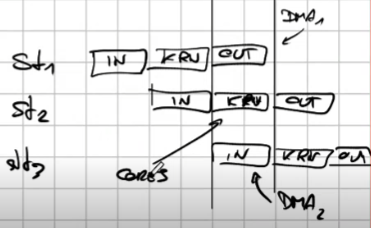
\includegraphics[scale=0.5]{24.png}
\end{center}
\end{multicols}
\pagebreak
\paragraph{Code example}
\begin{lstlisting}[style=myC]
#include <stdio.h>
#include <stdlib.h>
#include <time.h>

using namespace std;

void vecaddGPU(float *r, float *a, float *b, int n) {
	#pragma acc kernels loop copyin(a[0:n], b[0:n]) copyout(r[0:n])
	for (int i = 0; i < n; i++) r[0] = a[i] + b[i];
}

// note that the GPU memory is managed automatically and not explicitly by the programmer
int main(int argc, char* argv[]) {
	int n; // vector length
	float * a, * b, * r, * e; // inputs, output and expected vectors
	int i, errs;

	if (argc > 1) n = atoi(argv[1]);
	else n = 100000; // default vector length
	if (n <= 0) n = 100000;

	// allocate vectors on the CPU
	a = (float*) malloc(n*sizeof(float));
	b = (float*) malloc(n*sizeof(float));
	r = (float*) malloc(n*sizeof(float));
	e = (float*) malloc(n*sizeof(float));
	// populate vectors
	for (i = 0; i < n; i++) {
		a[i] = (float) i+1;
		b[i] = (float) 1000*i;
	}

	// compute on the GPU
	vecaddGPU(r, a, b, n);

	// compute on host to compare
	clock_t start = clock();
	for (i = 0; i < n; i++) e[i] = a[i] + b[i];
	clock_t stop = clock();
	printf("Seq time is: %f\n", ((double) (stop - start)/CLOCKS_PER_SEC));

	//compare results
	errs = 0;
	for (i = 0; i < n; i++) {
		if (r[i] != e[i]) errs++;
	}

	printf("%d errors found\n", errs);
	return errs;
}
\end{lstlisting}
\pagebreak
\paragraph{Kernels} Even with annotated code, where we don't have to write all the surrounding logic regarding the parallel computations, you have to be aware that you're executing a kernel which is a for loop of independent iterations.\\
Given some C code, which we want to turn into a kernel, it's relatively easy to turn into an AST (Abstract Syntax Tree). The we can take the list of variables and see those that are read before being written, those are plausibly the parameters we're getting from somewhere else, and those that are written and then never read anymore, which plausibly are the outputs to be reflected on the main memory.\\
You need a lot of code to \textbf{specify everything}. In particular three kinds of commands that you need to take into account:
\begin{list}{}{}
	\item Figure out the configuration of the board
	\item Define kernel
	\begin{list}{}{}
		\item OCL: compile a string, e.g. a file read from somewhere and with a specific command produce a kernel from the string that is directed to the GPU
		\item CUDA: special keywords that gets the code from the CUDA compiler, which is a wrapper on top of the C++ compiler
	\end{list}
	\item Direct command queue: copy out, copy in, kernel exec
\end{list}
OpenCL is both for CPU and GPU, so figuring out the config means how many cores on CPU too. On CPU, can do conditionals and divergent code in general, things you can't do on GPU.\\
OpenCL can be used for FPGAs too.
\subsection{FPGAs}
Devices with components that can be programmed to act as other components simply configuring them at the beginning, somehow. Basically: logical gates, small registers, small ALUs\ldots\\
A FPGA is an array where the single cell can act as if it were:
\begin{list}{}{}
	\item a small (5-7bit input and 1bit output) boolean network: made with a kind of EPROM which uses the input bits as an address and stores a single bit output
	\item a 1 bit register
	\item a router redirecting to a neighbor cell
\end{list}
The columns can host some RAM blocks, 1KB memory for intermediate values, or DSP blocks, basically multiplying addresses (multiply two inputs, adds the result with a register, stores the result of the addition in that register while propagating it too).\\
These are organized in columns so that there are columns composed solely of cells interleaved with RAM/DSP columns: a cells column may implement a certain function that stores the result in a RAM column, that may be routed in a way to do come floating point operations in a DSP column\ldots
\subparagraph{RTL} Register Transfer Level code used to program FPGA:
\begin{list}{}{}
	\item VHDL
	\item Verilog 
	
\begin{lstlisting}
module Name (input [N-1:0]x, input [N-1:0]y, output [N:0]z);
	// code example
	assign z = x + y; // creates a block which computes the sum and outputs in z
end module;
\end{lstlisting}
\end{list}
FPGAs are very good at executing pipelined code, with better performance than CPUs. For example $$\forall\:i\:\:a_i = b_i + c_i$$
a FPGA may operate with a memory interface able to load $a_i$ and $b_i$ into registers, then an adder which outputs to another register that delivers to a memory interface outputting $c_i$ in the memory. It costs a clock cycle per register level: first level of two registers, then adder and register and a final level with the memory interface which outputs $c_i$. Hence it costs 3 clock cycles.\\
On a CPU this would've took 2 loads, the add and the final store: 4 operations each of the fetch-decode-execute pipeline.\\\\
Also, this structure (which is a RAM column for the origin of $a_i,b_i$, a cells column for the memory interface, a DSP column for the add, another cells column for the memory interface and a final RAM column for the output $c_i$) can be easily replicated in multiple copies obtaining an hardware parallel computation of something already much faster than an original CPU code.
\begin{center}
	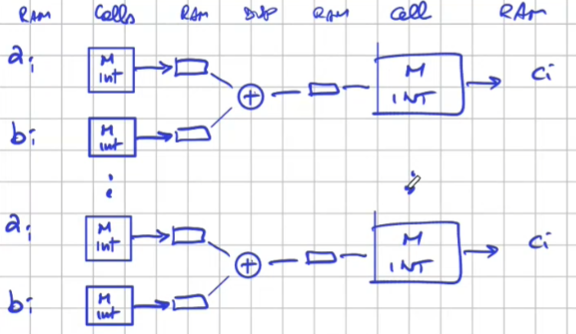
\includegraphics[scale=0.5]{25.png}
\end{center}
To achieve this you need a complex workflow which can go multiple ways. The classical is:
\begin{list}{}{}
	\item Write some RTL code
	\item Run the compiler, which solves many problems. In particular, FPGAs are graphs and a task is mapping between tasks which is NP-hard and may take hours to complete
	\item You get a bit stream file that we send to the FPGA (in configuration mode): is basically the entire configuration of the chip, and takes $\mu$seconds.
\end{list}
This is simplified, usually the RTL code is firstly run into simulators to check everything from performance to results.
\paragraph{Xilinx} Assumes a kernel code written in C with no pointers, no recursion\ldots and other limitations, filled with pragmas with calls to a library of components (e.g. communication channels to interconnect different kernels to a buffer in hardware). With HLS (High Level Synthesis) tools, the "compiler", you get the bit stream.\\
To operate the bitstream it's a different story. You have .ocl code where normally you have the \texttt{createProgram} with the GPU specified, that outputs a kernel that you can submit for execution in a queue, instead of the GPU you specify the bitstream obtained.\\
Then, you can run on the FPGA or simulate it on CPU/GPU.
\end{document}